\chapter{一阶方法}
\label{chap:first-order-methods}

设想站在一片山谷里，四周被雾遮住。每走到一处，只能用脚试出当地的坡度，也就是目标的函数值和梯度，看不到整个地形，也量不出地面的弯曲。这正是大规模优化最常见的处境：变量很多，Hessian算不起也存不下，一次梯度却是可以负担的。

本章全程使用同一个目标来比较各种走法：
\begin{equation}
 f(\bm{x})=\frac12\bigl(x_1^2+9x_2^2\bigr),\qquad
 \bm{x}^{(0)}=(9,1).
 \label{eq:fom-example}
\end{equation}
它的等高线是横向拉长的椭圆，最优解是原点。Hessian是$\bm{H}=\operatorname{diag}(1,9)$，所以$\mu=1$，$L=9$，$\kappa=9$。沿$x_1$方向地面平缓，沿$x_2$方向地面陡峭，这种“一个方向平、一个方向陡”的山谷称为病态的目标。

最朴素的走法是每步顺着最陡的方向下山。第~\ref{sec:fom-gradient-descent}节会看到，它在这个山谷里左右折返，大部分力气消耗在陡峭方向上。那么，能不能利用走过的路？第~\ref{sec:fom-momentum}节把上一步的位移加进当前更新，并比较梯度取在当前点和取在试探点这两种做法。第~\ref{sec:fom-ncg}节换一种用历史的方式：保留上一轮的搜索方向，与新梯度组合，再用线搜索决定走多远。

几种方法花费的计算不同，得到的保证也不同。有的保证只对二次目标成立，有的要求凸，有的只能说梯度变小。第~\ref{sec:fom-cost}节把它们放在同一把尺子下比较，并说明为什么迭代次数少不等于总计算少。

\section{梯度下降}
\label{sec:fom-gradient-descent}

只知道当前点的函数值和梯度，下一步应该朝哪里走、走多远？本节回答这个问题，并分三种情形说明这样走能得到什么：一般非凸、凸、强凸。三种情形的结论强弱不同，度量误差的尺子也不同。

\paragraph{主要思想}
先看方向。在$\bm{x}$附近，目标由一阶Taylor展开近似：
\[
 f(\bm{x}+\bm{d})\approx f(\bm{x})+\nabla f(\bm{x})^\top\bm{d}.
\]
在固定长度的$\bm{d}$中，要让$\nabla f(\bm{x})^\top\bm{d}$最小。由Cauchy--Schwarz不等式，
\[
 \nabla f(\bm{x})^\top\bm{d}\geq-\lVert\nabla f(\bm{x})\rVert_2\lVert\bm{d}\rVert_2,
\]
等号当且仅当$\bm{d}$与$-\nabla f(\bm{x})$同向时成立。所以局部最陡的下降方向是负梯度方向。

线性模型只给方向，不给距离：沿负梯度走得越远，线性模型的值越低，没有尽头。真实的地面会弯曲，线性预测走远了就不可信。需要一个量来说明“能信多远”。

这个量就是第~\ref{chap:smooth-foundations}章的光滑常数$L$，它要求梯度满足Lipschitz条件：
\[
 \lVert\nabla f(\bm{x})-\nabla f(\bm{y})\rVert_2\leq L\lVert\bm{x}-\bm{y}\rVert_2.
\]

在这个条件下，下降引理给出处处成立的二次上界：
\begin{equation}
 f(\bm{y})\leq f(\bm{x})+\nabla f(\bm{x})^\top(\bm{y}-\bm{x})+\frac{L}{2}\lVert\bm{y}-\bm{x}\rVert_2^2.
 \label{eq:fom-descent-lemma}
\end{equation}
二阶可微时，$\nabla^2f\preceq L\bm{I}$且$\nabla^2f\succeq-L\bm{I}$就保证了这一点。可以把右端想成扣在地面上的一只碗：它在$\bm{x}$处贴住地面，其余地方都不低于地面。

既然地面不高于这只碗，就走到碗底。对$\bm{y}$求右端的最小点，令导数为零，得到$\bm{y}=\bm{x}-\nabla f(\bm{x})/L$。图~\ref{fig:fom-upper-bound}画的是一元的情形：绿色的碗底对应的横坐标就是新点，碗底的高度保证了至少下降多少。

\begin{BookInlineFigure}
  \centering
  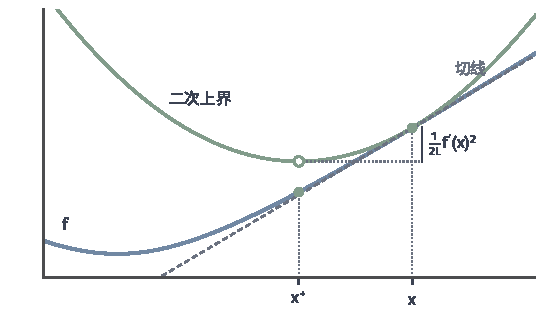
\includegraphics[width=92mm]{figures/05-optimization/02-smooth-optimization/matplotlib/fom-upper-bound/figure.pdf}
  \caption{二次上界决定一步走多远。蓝色曲线是$f(x)=\sqrt{1+x^2}$，它的二阶导数不超过$1$，取$L=1$。虚线是$x=2.4$处的切线，绿色抛物线是式~\eqref{eq:fom-descent-lemma}的上界。空心点是上界的最低点，其横坐标$x^{+}$就是新点，实心点是真实的函数值，它不高于空心点。竖线段是保证的下降量。}
  \label{fig:fom-upper-bound}
\end{BookInlineFigure}

把步长放宽为任意的$\alpha>0$，就得到\term{梯度下降法}（gradient descent method）：
\begin{equation}
 \bm{x}^{(t+1)}=\bm{x}^{(t)}-\alpha^{(t)}\bm{g}^{(t)},\qquad \bm{g}^{(t)}=\nabla f(\bm{x}^{(t)}).
 \label{eq:fom-gd}
\end{equation}
把$\bm{y}=\bm{x}^{(t+1)}$代入式~\eqref{eq:fom-descent-lemma}，一阶项是$-\alpha\lVert\bm{g}^{(t)}\rVert_2^2$，二次项是$\tfrac{L}{2}\alpha^2\lVert\bm{g}^{(t)}\rVert_2^2$，合起来得到单步下降估计：
\begin{equation}
 f(\bm{x}^{(t+1)})\leq f(\bm{x}^{(t)})-\alpha\Bigl(1-\frac{L\alpha}{2}\Bigr)\lVert\bm{g}^{(t)}\rVert_2^2.
 \label{eq:fom-gd-decrease}
\end{equation}
只要$0<\alpha<2/L$，括号就是正的，函数值严格下降。关于$\alpha$求最大的下降量，得到$\alpha=1/L$，此时每步至少下降$\lVert\bm{g}^{(t)}\rVert_2^2/(2L)$。

步长的来源有三种，都沿用第~\ref{chap:smooth-foundations}章的规则。已知$L$时取固定步长；不知道$L$时用回溯，从一个试探值开始不断缩短，直到满足Armijo条件
\begin{equation}
 f(\bm{x}+\alpha\bm{d})\leq f(\bm{x})+c_1\alpha\nabla f(\bm{x})^\top\bm{d},\qquad 0<c_1<1;
 \label{eq:fom-armijo}
\end{equation}
二次目标上还可以精确求沿线最小点。负梯度方向的精确步长是
\[
 \alpha=\frac{\bm{g}^\top\bm{g}}{\bm{g}^\top\bm{H}\bm{g}},
\]
这时的方法称为最速下降法（steepest descent）。

\needspace{6\baselineskip}
\paragraph{变量}
\begin{itemize}
 \item $\bm{x}^{(t)}\in\mathbb{R}^n$：当前点，在原处更新。
 \item $\bm{g}^{(t)}\in\mathbb{R}^n$：当前点的梯度，每轮读取一次。
 \item $\alpha>0$：步长，这里固定；用线搜索时每轮重新确定。
 \item $\varepsilon>0$，$T$：梯度大小的容差与最大步数。
\end{itemize}

\paragraph{初始化}
选定起点$\bm{x}^{(0)}$、步长、容差，令$t=0$。例中用式~\eqref{eq:fom-example}的起点，并取$\alpha=1/5$（下文说明这个值从哪里来），容差$\varepsilon=10^{-3}$。初始值是
\[
 \bm{x}^{(0)}=(9,1),\qquad f(\bm{x}^{(0)})=45.
\]

\needspace{6\baselineskip}
\paragraph{每轮更新}
在第$t$轮：
\begin{enumerate}
 \item \textbf{读取梯度。}计算$\bm{g}^{(t)}=\nabla f(\bm{x}^{(t)})$。例中$\nabla f(\bm{x})=(x_1,9x_2)$，第一轮
 \[
  \bm{g}^{(0)}=(9,9).
 \]
 \item \textbf{检查停止。}若$\lVert\bm{g}^{(t)}\rVert_2\leq\varepsilon$或$t=T$，输出$\bm{x}^{(t)}$并结束。例中第一轮$\lVert\bm{g}^{(0)}\rVert_2=9\sqrt2\approx12.73$，继续。
 \item \textbf{更新。}按式~\eqref{eq:fom-gd}计算新点，令$t\leftarrow t+1$。例中第一轮
 \[
  \bm{x}^{(1)}=(9,1)-\tfrac15(9,9)=(7.2,-0.8),\qquad f(\bm{x}^{(1)})=28.8.
 \]

 例中第二轮$\bm{g}^{(1)}=(7.2,-7.2)$，于是
 \[
  \bm{x}^{(2)}=(7.2,-0.8)-\tfrac15(7.2,-7.2)=(5.76,0.64),
 \]
 目标值$f(\bm{x}^{(2)})=18.432$。

 例中第三轮$\bm{g}^{(2)}=(5.76,5.76)$，于是
 \[
  \bm{x}^{(3)}=(5.76,0.64)-\tfrac15(5.76,5.76)=(4.608,-0.512),
 \]
 目标值$f(\bm{x}^{(3)})=11.79648$。
\end{enumerate}

规律已经显出来了：两个坐标分别乘以$1-\alpha\lambda$，第一个因子是$1-\tfrac15=0.8$，第二个因子是$1-\tfrac95=-0.8$。因此
\[
 \bm{x}^{(t)}=0.8^t\bigl(9,(-1)^t\bigr),\qquad f(\bm{x}^{(t)})=45\cdot0.64^t.
\]

梯度大小是$\lVert\bm{g}^{(t)}\rVert_2=0.8^t\cdot9\sqrt2$，它不超过$10^{-3}$要求$t\geq43$。最终得到
\[
 \bm{x}^{(43)}\approx(6.13\times10^{-4},\,-6.81\times10^{-5}).
\]
这个起点是特意选的：沿$\bm{d}=-\bm{g}$的精确步长恰好处处等于$1/5$，所以这串点也是最速下降的结果。

\paragraph{步长与收缩因子}
为什么取$1/5$，而不是上界推出的$1/L=1/9$？这要看二次目标上一步到底做了什么。设
\[
 f(\bm{x})=\frac12(\bm{x}-\bm{x}^\star)^\top\bm{H}(\bm{x}-\bm{x}^\star)+f^\star,
\]
其中$\bm{H}$对称正定，特征值都落在$[\mu,L]$内。记$\bm{e}^{(t)}=\bm{x}^{(t)}-\bm{x}^\star$，由$\bm{g}^{(t)}=\bm{H}\bm{e}^{(t)}$得
\[
 \bm{e}^{(t+1)}=(\bm{I}-\alpha\bm{H})\bm{e}^{(t)}.
\]

用$\bm{H}$的标准正交特征向量作坐标，矩阵变成对角形，每个特征方向各自演化。特征值为$\lambda$的分量每步乘以同一个数：
\begin{equation}
 e_\lambda^{(t+1)}=(1-\alpha\lambda)\,e_\lambda^{(t)}.
 \label{eq:fom-gd-factor}
\end{equation}
特征分解的做法可参考\BookChapterRef{chap:eigen-spectral-decomposition}{卷二第6章“谱分解”}。

步长是所有方向共用的一个数，而不同方向希望的步长不同：$\lambda$方向最想要$\alpha=1/\lambda$，一步到位。图~\ref{fig:fom-step-factor}把例中两个方向的因子画在一起。陡峭方向的折线下降得快，在$\alpha=1/9$处触底，随后反弹；平坦方向的线缓慢下降。整体的进度取决于两条线中较高的那条。

\begin{BookInlineFigure}
  \centering
  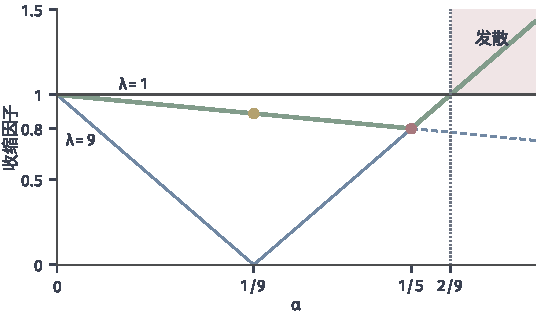
\includegraphics[width=92mm]{figures/05-optimization/02-smooth-optimization/matplotlib/fom-step-factor/figure.pdf}
  \caption{贯穿例上两个特征方向的收缩因子$\lvert1-\alpha\lambda\rvert$。蓝色实线对应陡峭方向$\lambda=9$，蓝色虚线对应平坦方向$\lambda=1$，绿色粗线是两者的较大值。黄点是$\alpha=1/L=1/9$，红点是使较大值最小的$\alpha=2/(L+\mu)=1/5$，此时因子等于$0.8$。红底区域$\alpha>2/9$中因子超过$1$，迭代发散。}
  \label{fig:fom-step-factor}
\end{BookInlineFigure}

要让最慢的方向尽量快，就让两条线相交。这件事可以写成一条定理。

\begin{theorem}[二次目标上的最佳固定步长]
\label{thm:fom-gd-quadratic}
设$\bm{H}$对称正定，特征值落在$[\mu,L]$内，且$\mu$和$L$都是特征值。固定步长的梯度下降收敛到$\bm{x}^\star$（对任意起点）当且仅当$0<\alpha<2/L$。取$\alpha=2/(L+\mu)$时，最大收缩因子最小，并且
\begin{equation}
 \lVert\bm{x}^{(t)}-\bm{x}^\star\rVert_2\leq\Bigl(\frac{\kappa-1}{\kappa+1}\Bigr)^t\lVert\bm{x}^{(0)}-\bm{x}^\star\rVert_2.
 \label{eq:fom-gd-quadratic-rate}
\end{equation}
\end{theorem}

\begin{proof}
由式~\eqref{eq:fom-gd-factor}，第$t$步的$\lambda$分量等于$(1-\alpha\lambda)^t$乘以初值。任意起点都收敛，当且仅当对每个特征值都有$\lvert1-\alpha\lambda\rvert<1$，即$0<\alpha\lambda<2$。这在$\lambda=L$时最严格，所以条件是$0<\alpha<2/L$。

函数$\lvert1-\alpha\lambda\rvert$关于$\lambda$是凸的，在$[\mu,L]$上的最大值在端点取得，所以最大因子是
\[
 \rho(\alpha)=\max\{\lvert1-\alpha\mu\rvert,\lvert1-\alpha L\rvert\}.
\]

随着$\alpha$增大，$1-\alpha\mu$减小，$\alpha L-1$增大。两者相等时最大值最小，这时$1-\alpha\mu=\alpha L-1$，解得
\[
 \alpha=\frac{2}{L+\mu},\qquad \rho=1-\frac{2\mu}{L+\mu}=\frac{\kappa-1}{\kappa+1}.
\]

最后，标准正交变换保持欧氏长度，各分量的平方和至多缩小$\rho^2$倍，即得结论。
\end{proof}

例中$\kappa=9$，$\rho=8/10=0.8$，正是上面算出的因子。起点$(9,1)$使两个方向同时达到这一因子，所以界~\eqref{eq:fom-gd-quadratic-rate}在这个例子上取等号。

图~\ref{fig:fom-gd-paths}把步长的影响画在等高线上。$\alpha=1/9$时第一步就消掉了$x_2$，随后沿谷底以因子$8/9$慢慢前进，路径光滑但慢；$\alpha=1/5$时路径左右折返，前进因子却是$0.8$；$\alpha=0.23$超过了$2/9$，$x_2$每步乘以$-1.07$，折返幅度越来越大。

\begin{BookInlineFigure}
  \centering
  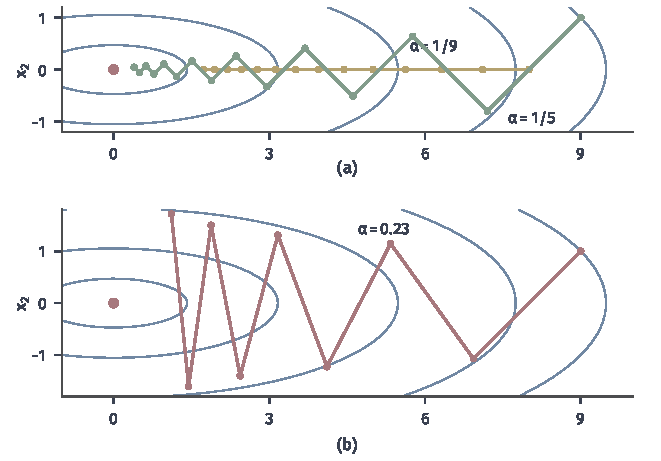
\includegraphics[width=112mm]{figures/05-optimization/02-smooth-optimization/matplotlib/fom-gd-paths/figure.pdf}
  \caption{贯穿例上不同固定步长的路径，蓝色椭圆是等高线，红点是最优解。(a)黄色路径$\alpha=1/9$，绿色路径$\alpha=1/5$，各走$14$步。(b)红色路径$\alpha=0.23>2/L$，走$8$步，$x_1$在收缩，$x_2$的振幅却在放大。}
  \label{fig:fom-gd-paths}
\end{BookInlineFigure}

于是$\alpha=1/L$与$\alpha=2/(L+\mu)$回答的是两个不同的问题。前者由上界推出，只用$L$，保证函数值每步下降，下面的定理都以它为基础；后者要同时知道$\mu$和$L$，它在二次目标上收缩最快，函数值也下降，但路径来回摆动。

\paragraph{一般非凸情形：梯度残差}
下面离开二次目标。先看最弱的假设：$f$可以非凸，只要求梯度Lipschitz，并且有下界。这时目标差和解距离都无从谈起，因为可能有许多局部的谷底，能评价的只有梯度的大小。

\begin{theorem}[非凸情形的梯度下降]
\label{thm:fom-gd-nonconvex}
设$f$的梯度$L$-Lipschitz连续，$f_{\inf}=\inf f>-\infty$。取固定步长$\alpha=1/L$，则对任意$T\geq1$，
\begin{equation}
 \min_{0\leq t<T}\lVert\bm{g}^{(t)}\rVert_2^2\leq\frac{2L\bigl(f(\bm{x}^{(0)})-f_{\inf}\bigr)}{T},
 \label{eq:fom-gd-nonconvex}
\end{equation}
并且$\lVert\bm{g}^{(t)}\rVert_2\to0$，$\{\bm{x}^{(t)}\}$的每个极限点都是驻点。
\end{theorem}

\begin{proof}
由式~\eqref{eq:fom-gd-decrease}，取$\alpha=1/L$时每步满足
\[
 \frac{1}{2L}\lVert\bm{g}^{(t)}\rVert_2^2\leq f(\bm{x}^{(t)})-f(\bm{x}^{(t+1)}).
\]

对$t=0,\ldots,T-1$求和，右端裂项，再用$f(\bm{x}^{(T)})\geq f_{\inf}$，得到
\[
 \frac{1}{2L}\sum_{t=0}^{T-1}\lVert\bm{g}^{(t)}\rVert_2^2\leq f(\bm{x}^{(0)})-f_{\inf}.
\]

$T$项的最小值不超过平均值，这就是式~\eqref{eq:fom-gd-nonconvex}。令$T\to\infty$，上式说明级数$\sum\lVert\bm{g}^{(t)}\rVert_2^2$收敛，所以通项趋于零。$\nabla f$连续，极限点处的梯度等于梯度序列的极限，也就是零。
\end{proof}

定理说的是“某一步的梯度够小”，并没有说最后一步最小，所以输出时要记住梯度最小的那个迭代点。换成任意$\alpha\in(0,2/L)$，只需把$1/(2L)$换成$\alpha(1-L\alpha/2)$。

用回溯时结论同样成立，只差常数。由式~\eqref{eq:fom-gd-decrease}，凡是$\alpha\leq2(1-c_1)/L$的步长都满足Armijo条件。所以若初始试探值为$\alpha_0$、每次缩短到$\rho$倍，接受的步长不低于$\min\{\alpha_0,2\rho(1-c_1)/L\}$，每步下降量有与上面同样形式的下界。

驻点不等于极小点。图~\ref{fig:fom-nonconvex}取非凸函数$f(\bm{x})=-\cos x_1+\tfrac92x_2^2$，它的Hessian是$\operatorname{diag}(\cos x_1,9)$，所以$L=9$，下确界是$-1$。从$(\pi,1)$出发的路径停在鞍点$(\pi,0)$，梯度为零，定理完全满足，点却不是局部最优解。稍稍偏开，从$(3,1)$出发，路径在鞍点附近徘徊一阵，再滑向真正的谷底。

\begin{BookInlineFigure}
  \centering
  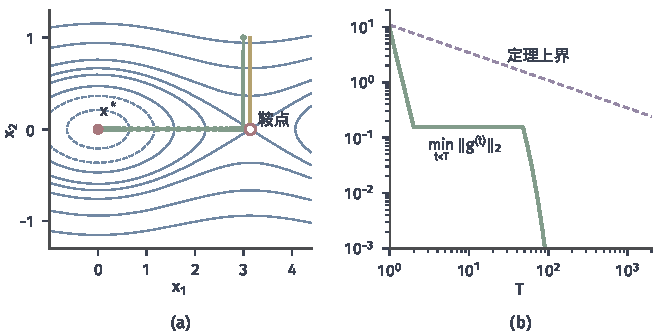
\includegraphics[width=112mm]{figures/05-optimization/02-smooth-optimization/matplotlib/fom-nonconvex/figure.pdf}
  \caption{非凸目标$f(\bm{x})=-\cos x_1+\tfrac92x_2^2$上取$\alpha=1/9$的梯度下降。(a)等高线与两条路径：黄色从$(\pi,1)$出发，终止于鞍点（红色空心点）；绿色从$(3,1)$出发，到达极小点（红点）。(b)绿色路径的$\min_{t<T}\lVert\bm{g}^{(t)}\rVert_2$（绿线），紫色虚线是式~\eqref{eq:fom-gd-nonconvex}的上界开方。中段的平台对应在鞍点附近的徘徊。}
  \label{fig:fom-nonconvex}
\end{BookInlineFigure}

\paragraph{凸情形：目标差}
加上凸性后，局部的谷底就是全局的谷底，可以用目标差来衡量。关键的新工具是：切平面从下方托住目标，用它比较当前点和最优解。

\begin{theorem}[凸情形的梯度下降]
\label{thm:fom-gd-convex}
设$f$凸，梯度$L$-Lipschitz连续，且存在最优解$\bm{x}^\star$。取$\alpha=1/L$，则对任意$T\geq1$，
\begin{equation}
 f(\bm{x}^{(T)})-f^\star\leq\frac{L\lVert\bm{x}^{(0)}-\bm{x}^\star\rVert_2^2}{2T}.
 \label{eq:fom-gd-convex}
\end{equation}
\end{theorem}

\begin{proof}
记$\bm{x}=\bm{x}^{(t)}$，$\bm{x}^+=\bm{x}^{(t+1)}$，$\bm{g}=\bm{g}^{(t)}$。由凸性，切平面在$\bm{x}^\star$处不高于目标：
\[
 f^\star\geq f(\bm{x})+\bm{g}^\top(\bm{x}^\star-\bm{x}).
\]

由式~\eqref{eq:fom-gd-decrease}，$\alpha=1/L$时单步下降至少为$\lVert\bm{g}\rVert_2^2/(2L)$。把上式代入，得到
\[
 f(\bm{x}^+)-f^\star\leq\bm{g}^\top(\bm{x}-\bm{x}^\star)-\frac{1}{2L}\lVert\bm{g}\rVert_2^2.
\]

把$\bm{x}^+=\bm{x}-\bm{g}/L$代入距离的平方，展开得
\[
 \lVert\bm{x}^+-\bm{x}^\star\rVert_2^2
 =\lVert\bm{x}-\bm{x}^\star\rVert_2^2-\frac2L\bm{g}^\top(\bm{x}-\bm{x}^\star)+\frac{1}{L^2}\lVert\bm{g}\rVert_2^2.
\]

两式比较，前一式的右端恰好等于距离平方之差的$L/2$倍：
\[
 f(\bm{x}^{(t+1)})-f^\star\leq\frac L2\Bigl(\lVert\bm{x}^{(t)}-\bm{x}^\star\rVert_2^2-\lVert\bm{x}^{(t+1)}-\bm{x}^\star\rVert_2^2\Bigr).
\]

对$t=0,\ldots,T-1$求和，右端裂项，丢掉末项，得到
\[
 \sum_{t=1}^{T}\bigl(f(\bm{x}^{(t)})-f^\star\bigr)\leq\frac L2\lVert\bm{x}^{(0)}-\bm{x}^\star\rVert_2^2.
\]

函数值逐步下降，所以最后一项是$T$项中最小的，不超过平均值，即得式~\eqref{eq:fom-gd-convex}。
\end{proof}

上面证明还顺带说明，到最优解的距离每步不增。

$1/T$这个阶对梯度下降不能改进。取$f(\bm{x})=\tfrac12(Lx_1^2+\lambda x_2^2)$，$0<\lambda\leq L$，起点的第一坐标为$0$，第二坐标为$x_0$。$\alpha=1/L$时目标差是$\tfrac12\lambda(1-\lambda/L)^{2T}x_0^2$。对每个给定的$T$，取$\lambda=L/(2T)$，因子$(1-1/(2T))^{2T}$接近$\mathrm{e}^{-1}$，于是目标差约为
\[
 \frac{Lx_0^2}{4\mathrm{e}\,T}.
\]
也就是说，曲率总可以小到让梯度下降在这$T$步内几乎察觉不到。这个例子的$\lambda$随$T$变化，它说明上界在整个函数类上的阶不能改进，并不是说某个固定的二次目标只有$1/T$的速度。

\paragraph{强凸情形：线性收敛}
再加上强凸，第~\ref{chap:optimization}章的结论告诉我们解存在且唯一。这时切平面之上还多出一个二次项：
\begin{equation}
 f(\bm{y})\geq f(\bm{x})+\nabla f(\bm{x})^\top(\bm{y}-\bm{x})+\frac\mu2\lVert\bm{y}-\bm{x}\rVert_2^2.
 \label{eq:fom-strong-convexity}
\end{equation}
这是一只从下方托住地面的碗，与式~\eqref{eq:fom-descent-lemma}从上方扣住地面的碗相对。上下两只碗夹住地形，每步的进度就能与当前的误差比较。

\begin{theorem}[强凸情形的梯度下降]
\label{thm:fom-gd-strong}
设$f$的梯度$L$-Lipschitz连续且满足式~\eqref{eq:fom-strong-convexity}，$\mu>0$，$\kappa=L/\mu$。取$\alpha=1/L$，则
\begin{equation}
 \begin{aligned}
 f(\bm{x}^{(T)})-f^\star&\leq\Bigl(1-\frac1\kappa\Bigr)^T\bigl(f(\bm{x}^{(0)})-f^\star\bigr),\\
 \lVert\bm{x}^{(T)}-\bm{x}^\star\rVert_2^2&\leq\Bigl(1-\frac1\kappa\Bigr)^T\lVert\bm{x}^{(0)}-\bm{x}^\star\rVert_2^2.
 \end{aligned}
 \label{eq:fom-gd-strong}
\end{equation}
\end{theorem}

\begin{proof}
先证梯度能控制目标差。在式~\eqref{eq:fom-strong-convexity}中对$\bm{y}$取右端的最小值，最小点是$\bm{y}=\bm{x}-\nabla f(\bm{x})/\mu$，于是
\[
 f^\star\geq f(\bm{x})-\frac{1}{2\mu}\lVert\nabla f(\bm{x})\rVert_2^2,
 \qquad\text{即}\qquad
 \lVert\nabla f(\bm{x})\rVert_2^2\geq2\mu\bigl(f(\bm{x})-f^\star\bigr).
\]

代入式~\eqref{eq:fom-gd-decrease}（$\alpha=1/L$），两边减去$f^\star$，得到
\[
 f(\bm{x}^+)-f^\star\leq\Bigl(1-\frac\mu L\Bigr)\bigl(f(\bm{x})-f^\star\bigr).
\]
迭代$T$次即得第一式。

再证距离。在式~\eqref{eq:fom-strong-convexity}中取$\bm{y}=\bm{x}^\star$，整理得
\[
 \bm{g}^\top(\bm{x}-\bm{x}^\star)\geq f(\bm{x})-f^\star+\frac\mu2\lVert\bm{x}-\bm{x}^\star\rVert_2^2.
\]

另由$f^\star\leq f(\bm{x}^+)$和单步下降，得到
\[
 \lVert\bm{g}\rVert_2^2\leq2L\bigl(f(\bm{x})-f^\star\bigr).
\]

把这两式代入距离平方的展开式：
\[
 \begin{aligned}
 \lVert\bm{x}^+-\bm{x}^\star\rVert_2^2
 &=\lVert\bm{x}-\bm{x}^\star\rVert_2^2-\frac2L\bm{g}^\top(\bm{x}-\bm{x}^\star)+\frac{1}{L^2}\lVert\bm{g}\rVert_2^2\\
 &\leq\Bigl(1-\frac\mu L\Bigr)\lVert\bm{x}-\bm{x}^\star\rVert_2^2-\frac2L\bigl(f(\bm{x})-f^\star\bigr)+\frac2L\bigl(f(\bm{x})-f^\star\bigr).
 \end{aligned}
\]
后两项抵消，迭代$T$次即得第二式。
\end{proof}

用贯穿例核对。$\alpha=1/9$时$\bm{x}^{(1)}=(8,0)$，此后第一坐标每步乘以$8/9$，所以
\[
 f(\bm{x}^{(T)})=32\Bigl(\frac{64}{81}\Bigr)^{T-1},\qquad T\geq1.
\]
定理的上界是$45\cdot(8/9)^T$，$T=1$时是$40$，大于真实值$32$。图~\ref{fig:fom-gd-rates}(a)显示，上界比真实的衰减慢：定理覆盖所有满足条件的函数，这个二次例子并不是最坏的。

\paragraph{条件数怎样影响进展}
三条定理合起来回答了“要多少步”。目标差达到$\varepsilon$所需的步数，凸时约为$LR^2/(2\varepsilon)$，其中$R=\lVert\bm{x}^{(0)}-\bm{x}^\star\rVert_2$；强凸时由$(1-1/\kappa)^T\leq\mathrm{e}^{-T/\kappa}$得到
\[
 T\geq\kappa\ln\frac{f(\bm{x}^{(0)})-f^\star}{\varepsilon}.
\]

所需步数与$\kappa$成正比。把山谷的纵横比拉大十倍，步数也大约变成十倍。图~\ref{fig:fom-gd-rates}(b)对$\operatorname{diag}(1,\kappa)$实测目标差降到初值$10^{-6}$的步数，它紧贴直线$\tfrac\kappa4\ln(1/\varepsilon)$。这里$\tfrac14$来自最佳步长：因子$(\kappa-1)/(\kappa+1)$约为$1-2/\kappa$，目标差的因子是其平方。

\begin{BookInlineFigure}
  \centering
  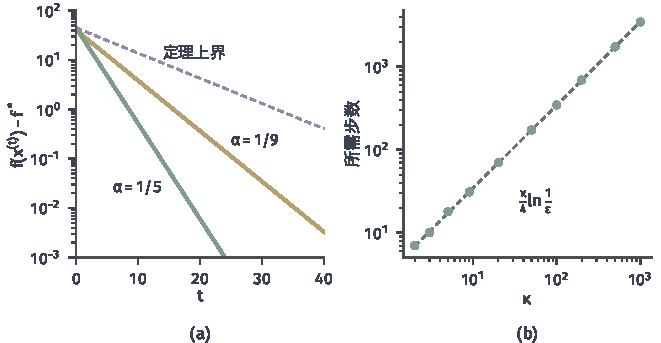
\includegraphics[width=112mm]{figures/05-optimization/02-smooth-optimization/matplotlib/fom-gd-rates/figure.pdf}
  \caption{收敛速度与条件数。(a)贯穿例的目标差：黄线$\alpha=1/9$，绿线$\alpha=1/5$，紫色虚线是$\alpha=1/L$时式~\eqref{eq:fom-gd-strong}的上界$45(8/9)^t$。(b)目标$\tfrac12(x_1^2+\kappa x_2^2)$，起点$(\kappa,1)$，步长$2/(1+\kappa)$，绿点是目标差降到初值$10^{-6}$倍的实测步数，虚线为$\tfrac\kappa4\ln(1/\varepsilon)$，$\varepsilon=10^{-6}$。}
  \label{fig:fom-gd-rates}
\end{BookInlineFigure}

原因已经在式~\eqref{eq:fom-gd-factor}中：步长被陡峭方向限制在$2/L$以内，平坦方向每步只能收缩$\mu/L$量级的比例。下面的表格汇总三种情形。

\begin{BookInlineTable}
  \centering
  \caption{梯度下降$\alpha=1/L$的保证，$\Delta=f(\bm{x}^{(0)})-f_{\inf}$，$R=\lVert\bm{x}^{(0)}-\bm{x}^\star\rVert_2$。}
  \label{tab:fom-gd-summary}
  \begin{tabular}{llll}
   \toprule
   假设 & 度量 & 上界 & 达到$\varepsilon$的步数\\
   \midrule
   非凸，有下界 & $\min_t\lVert\bm{g}^{(t)}\rVert_2^2$ & $2L\Delta/T$ & $2L\Delta/\varepsilon$\\
   凸 & $f(\bm{x}^{(T)})-f^\star$ & $LR^2/(2T)$ & $LR^2/(2\varepsilon)$\\
   强凸 & $f(\bm{x}^{(T)})-f^\star$ & $(1-1/\kappa)^T\Delta$ & $\kappa\ln(\Delta/\varepsilon)$\\
   \bottomrule
  \end{tabular}
\end{BookInlineTable}

表中第一行的$\varepsilon$是梯度平方的容差，所以换成梯度大小达到$\varepsilon$时，步数是$2L\Delta/\varepsilon^2$。三行的度量不同，步数不能直接相比。

\section{动量与加速}
\label{sec:fom-momentum}

上一节的结论是：病态目标上梯度下降的步数与$\kappa$成正比。不增加每步的梯度读取次数，只多用一点历史信息，能不能把这个依赖关系变小？

先看贯穿例上折返时发生了什么。图~\ref{fig:fom-zigzag}(a)把$\alpha=1/5$的每步位移分解到两个坐标。平坦方向$x_1$上，每一步的位移都向负方向，符号一致；陡峭方向$x_2$上，位移的符号每步翻转，走过去又走回来，大部分抵消。

\begin{BookInlineFigure}
  \centering
  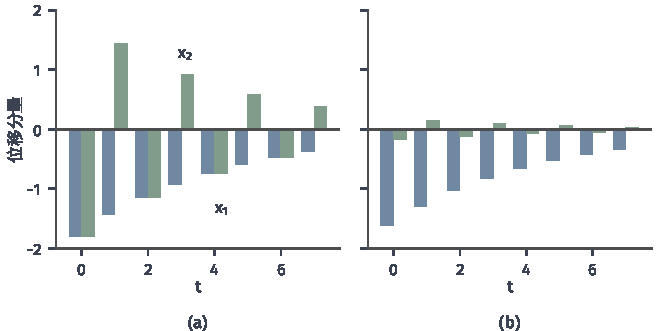
\includegraphics[width=112mm]{figures/05-optimization/02-smooth-optimization/matplotlib/fom-zigzag/figure.pdf}
  \caption{贯穿例上$\alpha=1/5$的梯度下降的位移。蓝色条是平坦方向$x_1$的分量，绿色条是陡峭方向$x_2$的分量。(a)每一步的位移$\bm{x}^{(t+1)}-\bm{x}^{(t)}$，绿色条的符号逐步交替。(b)相邻两步位移的平均，绿色条几乎消失，蓝色条保持不变的符号与相近的大小。}
  \label{fig:fom-zigzag}
\end{BookInlineFigure}

图~\ref{fig:fom-zigzag}(b)把相邻两步取平均：振荡方向互相抵消，一致方向得以保留。这就是用历史信息的线索：过去的位移本身携带了“哪些方向一直在走、哪些方向在来回”的信息，而这一信息不用额外计算梯度。

把上一步的位移乘一个系数加进当前更新，这个附加量称为\term{动量}（momentum）。下面两个方法都用动量，差别在梯度取在什么地方：重球法取在当前点，Nesterov方法取在沿动量向前试探的点。

\subsection{Polyak重球法}
\label{sec:fom-heavy-ball}

\paragraph{主要思想}
想象一个有质量的球在山谷中滚动，并受到摩擦。球的速度不会突然改变：沿谷底方向的重力持续推动，它越滚越快；沿谷壁方向的重力来回变号，速度被平均掉了。这就是想要的效果。

类比可以写成方程。位置$\bm{x}(\tau)$满足
\[
 \ddot{\bm{x}}+a\dot{\bm{x}}+\nabla f(\bm{x})=\bm{0},
\]
其中$a>0$是摩擦系数。用步长$h$的差分代替导数：
\[
 \ddot{\bm{x}}\approx\frac{\bm{x}^{(t+1)}-2\bm{x}^{(t)}+\bm{x}^{(t-1)}}{h^2},\qquad
 \dot{\bm{x}}\approx\frac{\bm{x}^{(t)}-\bm{x}^{(t-1)}}{h}.
\]

代入方程并整理，得到\term{重球法}（heavy ball method）\scite{polyak1964heavyball}：
\begin{equation}
 \bm{x}^{(t+1)}=\bm{x}^{(t)}-\alpha\bm{g}^{(t)}+\beta\bigl(\bm{x}^{(t)}-\bm{x}^{(t-1)}\bigr),
 \label{eq:fom-hb}
\end{equation}
其中$\alpha=h^2$，$\beta=1-ah$。摩擦越小，$\beta$越接近$1$，历史保留得越多。类比只解释了公式的样子，它并不提供收敛保证：离散的步子可以跨过谷底，下面会看到这确实造成困难。

$\alpha$和$\beta$怎样选？在正定二次目标上可以精确分析。与梯度下降一样，取$\bm{H}$的特征方向作坐标，由式~\eqref{eq:fom-hb}，特征值$\lambda$对应的误差分量满足二阶递推
\begin{equation}
 e_\lambda^{(t+1)}=(1+\beta-\alpha\lambda)e_\lambda^{(t)}-\beta e_\lambda^{(t-1)}.
 \label{eq:fom-hb-scalar}
\end{equation}

二阶线性递推的行为由特征方程的两个根决定：
\begin{equation}
 r^2-(1+\beta-\alpha\lambda)r+\beta=0.
 \label{eq:fom-hb-char}
\end{equation}
两根之积是$\beta$。判别式小于零时两根共轭，模相等，所以模都等于$\sqrt\beta$，\emph{与$\lambda$无关}。这是重球法最关键的现象：梯度下降的因子$1-\alpha\lambda$随方向变化，动量却可以把一段特征值的收缩速度拉平。

判别式小于等于零，就是$\lvert1+\beta-\alpha\lambda\rvert\leq2\sqrt\beta$。把它拆成上下两个不等式，并用$1+\beta\mp2\sqrt\beta=(1\mp\sqrt\beta)^2$，得到
\begin{equation}
 (1-\sqrt\beta)^2\leq\alpha\lambda\leq(1+\sqrt\beta)^2.
 \label{eq:fom-hb-complex}
\end{equation}
落在这个区间内的$\lambda$，收缩因子都是$\sqrt\beta$；落在区间外时两根是实数，积为$\beta$，其中一个的绝对值大于$\sqrt\beta$，收缩变慢。

于是设计问题变得清楚：让$[\alpha\mu,\alpha L]$全部落入区间~\eqref{eq:fom-hb-complex}，同时让$\sqrt\beta$尽量小。$\beta$越小区间越窄，所以最优时区间的两端恰好卡住，
\[
 (1-\sqrt\beta)^2=\alpha\mu,\qquad(1+\sqrt\beta)^2=\alpha L.
\]

两式开方后相除，得到$\sqrt\kappa=(1+\sqrt\beta)/(1-\sqrt\beta)$，解出$\sqrt\beta$；两式开方后相加，得到$\sqrt{\alpha L}+\sqrt{\alpha\mu}=2$，解出$\alpha$。结果是
\begin{equation}
 \alpha=\frac{4}{(\sqrt L+\sqrt\mu)^2},\qquad
 \beta=\Bigl(\frac{\sqrt\kappa-1}{\sqrt\kappa+1}\Bigr)^2.
 \label{eq:fom-hb-params}
\end{equation}
收缩因子$\sqrt\beta=(\sqrt\kappa-1)/(\sqrt\kappa+1)$的形式与梯度下降相同，只是$\kappa$换成了$\sqrt\kappa$。

例中$L=9$，$\mu=1$，$\sqrt\kappa=3$，所以
\[
 \alpha=\frac{4}{(3+1)^2}=\frac14,\qquad\beta=\Bigl(\frac24\Bigr)^2=\frac14,\qquad\sqrt\beta=\frac12.
\]

图~\ref{fig:fom-hb-roots}(a)画出$\lambda$从$1$走到$9$时根的运动。$\lambda=1$时是实轴上的二重根$\tfrac12$，随着$\lambda$增大，两根沿半径$\tfrac12$的圆分开，在$\lambda=5$时到达$\pm\tfrac12\mathrm{i}$，再在$\lambda=9$时汇合于$-\tfrac12$。梯度下降的单根则在实轴上从$0.8$移动到$-0.8$。图~\ref{fig:fom-hb-roots}(b)把模按$\lambda$展开：梯度下降是V形，重球法是平底。

\begin{BookInlineFigure}
  \centering
  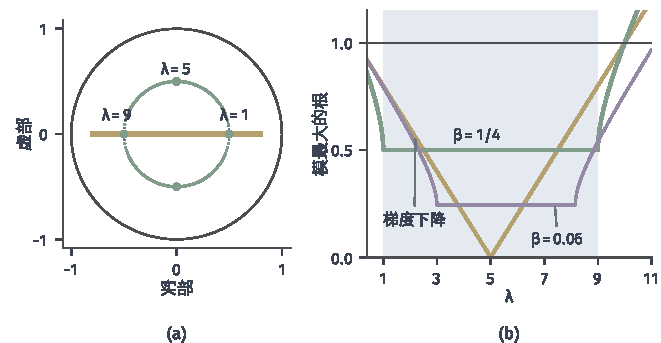
\includegraphics[width=112mm]{figures/05-optimization/02-smooth-optimization/matplotlib/fom-hb-roots/figure.pdf}
  \caption{重球法的特征根。(a)$\alpha=\beta=1/4$时，$\lambda\in[1,9]$对应的根（绿色）落在半径$1/2$的圆上；黄色线段是$\alpha=1/5$的梯度下降的根$1-\alpha\lambda$；外圈是单位圆。(b)模最大的根关于$\lambda$的变化，蓝底区间是$[\mu,L]$。绿线$\alpha=\beta=1/4$的平底宽度正好覆盖$[1,9]$；黄线是$\alpha=1/5$的梯度下降；紫线取$\alpha=0.19$，$\beta=0.06$，平底变低却变窄，靠近区间两端时被实根抬高。}
  \label{fig:fom-hb-roots}
\end{BookInlineFigure}

\needspace{6\baselineskip}
\paragraph{变量}
\begin{itemize}
 \item $\bm{x}^{(t)},\bm{x}^{(t-1)}\in\mathbb{R}^n$：当前点与上一点，比梯度下降多存一个向量。
 \item $\bm{g}^{(t)}\in\mathbb{R}^n$：当前点的梯度。
 \item $\alpha>0$，$0\leq\beta<1$：步长与动量系数，全程固定。
 \item $\varepsilon$，$T$：容差与最大步数。
\end{itemize}

\paragraph{初始化}
规定$\bm{x}^{(-1)}=\bm{x}^{(0)}$，于是第一步没有动量，就是一步梯度下降。按式~\eqref{eq:fom-hb-params}确定参数。例中$\alpha=\beta=1/4$，容差$\varepsilon=10^{-3}$，起点仍是
\[
 \bm{x}^{(-1)}=\bm{x}^{(0)}=(9,1).
\]

\needspace{6\baselineskip}
\paragraph{每轮更新}
在第$t$轮：
\begin{enumerate}
 \item \textbf{读取梯度并检查停止。}计算$\bm{g}^{(t)}$；若$\lVert\bm{g}^{(t)}\rVert_2\leq\varepsilon$或$t=T$，输出$\bm{x}^{(t)}$。例中第一轮
 \[
  \bm{g}^{(0)}=(9,9),\qquad\lVert\bm{g}^{(0)}\rVert_2\approx12.73.
 \]
 \item \textbf{计算动量项。}令$\bm{m}^{(t)}=\beta(\bm{x}^{(t)}-\bm{x}^{(t-1)})$。例中第一轮
 \[
  \bm{m}^{(0)}=\bm{0}.
 \]
 \item \textbf{更新。}按式~\eqref{eq:fom-hb}把负梯度步和动量项加到$\bm{x}^{(t)}$上，令$t\leftarrow t+1$。例中第一轮
 \[
  \bm{x}^{(1)}=(9,1)-\tfrac14(9,9)=(6.75,-1.25),\qquad f(\bm{x}^{(1)})=29.8125.
 \]

 例中第二轮，梯度和动量项分别是
 \[
  \bm{g}^{(1)}=(6.75,-11.25),\qquad\bm{m}^{(1)}=\tfrac14(-2.25,-2.25)=(-0.5625,-0.5625),
 \]
 于是
 \[
  \bm{x}^{(2)}=(6.75,-1.25)-(1.6875,-2.8125)+(-0.5625,-0.5625)=(4.5,1),
 \]
 $f(\bm{x}^{(2)})=14.625$。

 例中第三轮，梯度和动量项分别是
 \[
  \bm{g}^{(2)}=(4.5,9),\qquad\bm{m}^{(2)}=\tfrac14(-2.25,2.25)=(-0.5625,0.5625),
 \]
 于是
 \[
  \bm{x}^{(3)}=(4.5,1)-(1.125,2.25)+(-0.5625,0.5625)=(2.8125,-0.6875),
 \]
 $f(\bm{x}^{(3)})\approx6.082$。比较梯度下降的第三步$f\approx11.80$，已经差了将近一半。
\end{enumerate}

在这个例子上，式~\eqref{eq:fom-hb-char}的根是二重的：$\lambda=1$时为$\tfrac12$，$\lambda=9$时为$-\tfrac12$。二重根的递推解是$(a+bt)r^t$，由前两项定出系数，两个坐标是
\begin{equation}
 x_1^{(t)}=\frac{9+4.5t}{2^t},\qquad x_2^{(t)}=(1+1.5t)\Bigl(-\frac12\Bigr)^t.
 \label{eq:fom-hb-closed}
\end{equation}

代入$t=19$，梯度大小约为$5.4\times10^{-4}$，$t=18$时仍大于$10^{-3}$，于是第$19$步满足容差并结束。最终得到
\[
 \bm{x}^{(19)}\approx(1.80\times10^{-4},\,-5.63\times10^{-5}).
\]
同样的容差，梯度下降$\alpha=1/5$需要$43$步。

\paragraph{二次目标上的收敛}
式~\eqref{eq:fom-hb-closed}中的$1+1.5t$值得留意：根是二重时，收敛并不是纯粹的$\rho^t$，前面还有一个线性增长的因子。下面的定理把它显式写出来。

\begin{theorem}[正定二次目标上的重球法]
\label{thm:fom-hb-quadratic}
设$f$是Hessian为$\bm{H}$的二次目标，最优解为$\bm{x}^\star$，$\bm{H}$对称正定，特征值落在$[\mu,L]$内，$\kappa=L/\mu>1$。按式~\eqref{eq:fom-hb-params}取参数，令$\bm{x}^{(-1)}=\bm{x}^{(0)}$，$\rho=(\sqrt\kappa-1)/(\sqrt\kappa+1)$，则
\begin{equation}
 \lVert\bm{x}^{(t)}-\bm{x}^\star\rVert_2\leq(2t+1)\rho^t\lVert\bm{x}^{(0)}-\bm{x}^\star\rVert_2.
 \label{eq:fom-hb-rate}
\end{equation}
\end{theorem}

\begin{proof}
由式~\eqref{eq:fom-hb-complex}及参数的取法，每个特征值对应的两根$r_1,r_2$的模都等于$\rho$，并且$r_1+r_2=1+\beta-\alpha\lambda$，$r_1r_2=\beta=\rho^2$。

定义$S_k=\sum_{j=0}^kr_1^jr_2^{k-j}$，规定$S_{-1}=0$。由定义有$S_{k+1}=r_1S_k+r_2^{k+1}$，同理$S_k=r_1S_{k-1}+r_2^k$。把第二式乘以$r_2$后代入第一式，得到
\[
 S_{k+1}=(r_1+r_2)S_k-r_1r_2S_{k-1}.
\]

所以$S_t$满足递推~\eqref{eq:fom-hb-scalar}。分量的解可以写成$e^{(t)}=S_te^{(0)}-\beta S_{t-1}e^{(-1)}$：它满足同一递推，而$t=0$和$t=1$时分别等于$e^{(0)}$和式~\eqref{eq:fom-hb-scalar}的右端。

由$e^{(-1)}=e^{(0)}$，$\lvert S_k\rvert\leq(k+1)\rho^k$和$\beta=\rho^2$，
\[
 \lvert e^{(t)}\rvert\leq\bigl((t+1)\rho^t+\rho^2\,t\,\rho^{t-1}\bigr)\lvert e^{(0)}\rvert\leq(2t+1)\rho^t\lvert e^{(0)}\rvert,
\]
最后一步用了$\rho<1$。对所有特征方向平方求和，再用标准正交变换保持长度，即得结论。
\end{proof}

证明中间一步的界是$(t+1+\rho t)\rho^t$。例中$\rho=\tfrac12$，第二坐标恰好取到这个界，即$(1+1.5t)2^{-t}$，与式~\eqref{eq:fom-hb-closed}相符。图~\ref{fig:fom-hb-paths}(b)展示了多项式因子的后果：比值$x_2^{(t)}/x_2^{(0)}$第一步到达$-1.25$，比初值还大，随后才在紫色包络线外侧逐渐衰减。

\begin{BookInlineFigure}
  \centering
  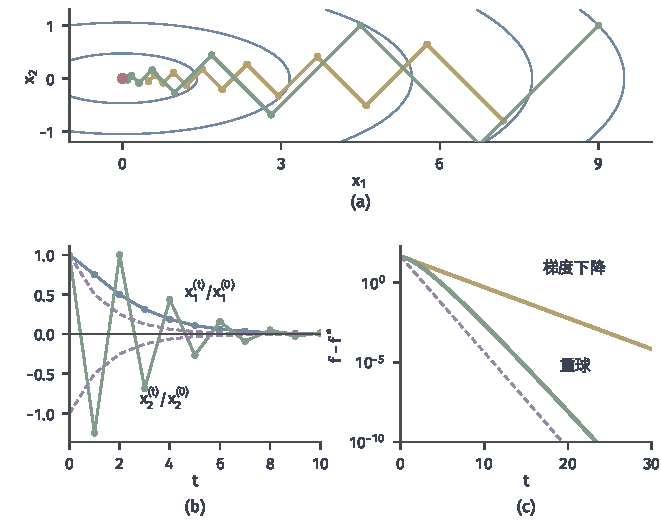
\includegraphics[width=112mm]{figures/05-optimization/02-smooth-optimization/matplotlib/fom-hb-paths/figure.pdf}
  \caption{贯穿例上的重球法（绿色，$\alpha=\beta=1/4$）与梯度下降（黄色，$\alpha=1/5$）。(a)等高线上的前$14$步。(b)重球法两坐标相对初值的比，式~\eqref{eq:fom-hb-closed}，紫色虚线是$\pm\rho^t$。(c)目标差的半对数曲线，紫色虚线是$45\rho^{2t}$，绿线在上方平行，差别来自多项式因子。}
  \label{fig:fom-hb-paths}
\end{BookInlineFigure}

所以，用$\rho$比较两种方法时，要记住它是渐近的说法。达到相对精度$\varepsilon$的步数约为$\tfrac{\sqrt\kappa}{2}\ln(1/\varepsilon)$，与梯度下降的$\tfrac\kappa2\ln(1/\varepsilon)$相比，$\kappa=10^4$时大约快一百倍。

\paragraph{参数的稳定范围}
这个加速依赖于参数对$L$和$\mu$的准确了解。由递推~\eqref{eq:fom-hb-scalar}的两根都在单位圆内的条件，可以写出稳定范围。多项式$p(r)=r^2-(1+\beta-\alpha\lambda)r+\beta$满足$p(1)=\alpha\lambda$，$p(-1)=2(1+\beta)-\alpha\lambda$，在$\beta\geq0$时，两根都在单位圆内当且仅当
\begin{equation}
 \beta<1,\qquad0<\alpha\lambda<2(1+\beta).
 \label{eq:fom-hb-stable}
\end{equation}

判据是$p(1)>0$，$p(-1)>0$，且根之积$\beta$的绝对值小于$1$。例中若沿用$\alpha=1/4$，却把$\beta$减到$0.06$，则$\alpha L=2.25$大于$2(1+\beta)=2.12$，陡峭方向发散。动量不只是“加速的旋钮”，它也放宽了步长的稳定界限，两个参数必须一起调。

\paragraph{离开二次目标}
式~\eqref{eq:fom-hb-params}的推导完全依赖于每个方向有固定的$\lambda$。目标不是二次时，局部曲率随位置变化，没有固定的特征方向。若$f$二阶连续可微，而$\bm{x}^\star$处的Hessian特征值落在$[\mu,L]$内，在$\bm{x}^\star$足够近处迭代可以用线性化来分析，局部收敛速度接近$\rho$；这是局部结论，对起点有要求。

全局情形下，这组参数确实可能失败。考虑一元函数，其导数分三段：
\begin{equation}
 f'(x)=\begin{cases}
 25x,&x<1,\\
 x+24,&1\leq x<2,\\
 25x-24,&x\geq2.
 \end{cases}
 \label{eq:fom-hb-counterexample}
\end{equation}
三段在分界点处衔接，$f'$连续且斜率都在$[1,25]$内，所以$f$强凸，$\mu=1$，$L=25$，最优解是$x^\star=0$。二次目标的最优参数是$\alpha=1/9$，$\beta=4/9$。

这组参数有一个周期为$3$的轨道，不会收敛：
\[
 x\text{ 依次取}\quad \frac{792}{1225},\quad-\frac{2208}{1225},\quad\frac{2592}{1225}.
\]

可以逐步核对。从前两点$2592/1225$（上一点）和$792/1225$（当前点）出发，当前点小于$1$，导数是$25x$。代入式~\eqref{eq:fom-hb}并把分母提出来：
\[
 x^{+}=\frac{1}{1225}\Bigl(792-\frac{25\cdot792}{9}+\frac49(792-2592)\Bigr)=-\frac{2208}{1225}.
\]

下一步当前点$-2208/1225$仍小于$1$，同样算得$2592/1225$。再下一步，当前点约为$2.116$，落在第三段，导数$25x-24$多出的常数$-24$提供了回拉，算得的新点恰好回到$792/1225$。

图~\ref{fig:fom-hb-cycle}展示了$x^{(0)}=3.3$时的情形：迭代很快落到这个周期上。作为对照，下一小节的方法在同一函数上正常收敛。这个反例说明，正定二次目标上的最优参数不能直接移到一般强凸目标上，也不能因此宣称全局加速。

\begin{BookInlineFigure}
  \centering
  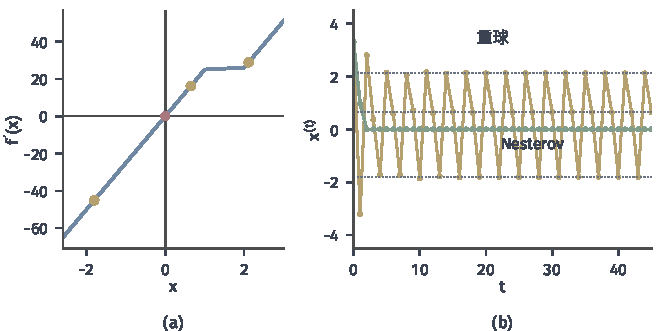
\includegraphics[width=112mm]{figures/05-optimization/02-smooth-optimization/matplotlib/fom-hb-cycle/figure.pdf}
  \caption{强凸光滑目标上重球法不收敛的例子。(a)式~\eqref{eq:fom-hb-counterexample}的导数$f'(x)$（蓝线），红点是最优解，黄点是周期轨道的三个点。(b)从$x^{(0)}=3.3$出发的迭代，黄线是重球法（$\alpha=1/9$，$\beta=4/9$），落到灰色点线标出的周期上；绿线是$\alpha=1/25$，$\beta=2/3$的Nesterov方法，收敛到$0$。}
  \label{fig:fom-hb-cycle}
\end{BookInlineFigure}

对一般强凸目标，缩小参数可以恢复全局收敛，但已知的这类分析一般达不到$\sqrt\kappa$的依赖，具体的条件和常数需要逐项核对，证明较长，读者可查阅一阶方法的专门文献。本章只在正定二次目标上给重球法下定量结论。

\subsection{Nesterov加速梯度法}
\label{sec:fom-nesterov}

\paragraph{主要思想}
重球法的动量盲目地累加：梯度在当前点读取，动量推出的位置却没有被检查，步子跨过谷底时也不会被纠正。一个自然的改进是把两件事的次序换一下：先顺着动量探出去，到探出的位置上再看坡度，用那里的梯度来修正。

这就是\term{Nesterov加速梯度法}（Nesterov accelerated gradient）\scite{nesterov1983method}。

它先由当前与历史迭代构成\term{外推点}（extrapolation point）$\bm{y}^{(t)}$，再在外推点做一步梯度下降：
\begin{equation}
 \begin{aligned}
 \bm{y}^{(t)}&=\bm{x}^{(t)}+\beta^{(t)}\bigl(\bm{x}^{(t)}-\bm{x}^{(t-1)}\bigr),\\
 \bm{x}^{(t+1)}&=\bm{y}^{(t)}-\alpha\nabla f(\bm{y}^{(t)}).
 \end{aligned}
 \label{eq:fom-nag}
\end{equation}
与式~\eqref{eq:fom-hb}比较，只有梯度的计算位置不同。图~\ref{fig:fom-nag-geometry}把一步的结构并排画出。

\begin{BookInlineFigure}
  \centering
  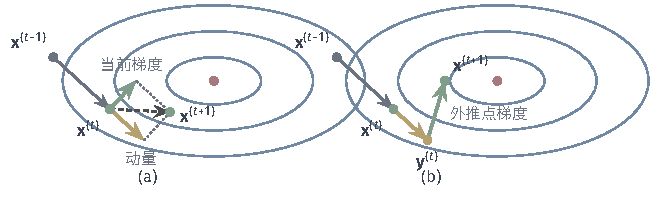
\includegraphics[width=110mm]{figures/05-optimization/02-smooth-optimization/tikz/fom-nag-geometry/figure.pdf}
  \caption{一步更新的结构对比，蓝色椭圆是等高线，红点是最优解。(a)重球法：动量（黄）和当前点的负梯度（绿）都从$\bm{x}^{(t)}$出发，两者相加得到新点。(b)Nesterov方法：先沿动量走到外推点$\bm{y}^{(t)}$，再从那里走一步负梯度。外推点已经冲到谷壁的外侧，那里的梯度把步子拉回。}
  \label{fig:fom-nag-geometry}
\end{BookInlineFigure}

用二次目标看这一改变的效果。代入$\nabla f(\bm{y})=\bm{H}(\bm{y}-\bm{x}^\star)$，并在特征方向上写开，记$s=1-\alpha\lambda$，得到
\begin{equation}
 e_\lambda^{(t+1)}=s\Bigl((1+\beta)e_\lambda^{(t)}-\beta e_\lambda^{(t-1)}\Bigr).
 \label{eq:fom-nag-scalar}
\end{equation}

对照式~\eqref{eq:fom-hb-scalar}。重球法的$-\beta e^{(t-1)}$不受$\lambda$影响，动量对各方向一视同仁；这里动量也被乘了$s$，曲率大的方向$s$小，动量被自动压低。这就是“外推点的梯度纠正动量”在公式上的含义。

特征方程是$r^2-s(1+\beta)r+s\beta=0$。复根时两根的积等于模的平方，所以模是$\sqrt{s\beta}$，随$\lambda$的增大而减小。

参数怎样选？取$\alpha=1/L$。例如强凸时取
\begin{equation}
 \beta=\frac{\sqrt\kappa-1}{\sqrt\kappa+1}.
 \label{eq:fom-nag-beta-strong}
\end{equation}
于是最平坦的方向$\lambda=\mu$上，$s=1-1/\kappa$，判别式恰好为零，二重根是$1-1/\sqrt\kappa$。由$(1+\beta)^2s=4\beta$可以直接验证这一点：把$\beta$代入，$(1+\beta)=2\sqrt\kappa/(\sqrt\kappa+1)$，$4\beta/(1+\beta)^2=(\kappa-1)/\kappa=s$。

而光滑凸时，$\mu$不可用，系数要随步数增长，后文的定理将说明它的具体形式。例中$\sqrt\kappa=3$，
\[
 \alpha=\frac19,\qquad\beta=\frac12,\qquad1-\frac{1}{\sqrt\kappa}=\frac23.
\]

\needspace{6\baselineskip}
\paragraph{变量}
\begin{itemize}
 \item $\bm{x}^{(t)},\bm{x}^{(t-1)}\in\mathbb{R}^n$：当前点与上一点。
 \item $\bm{y}^{(t)}\in\mathbb{R}^n$：外推点，梯度在这里读取，用后可覆盖。
 \item $\alpha$，$\beta^{(t)}$：步长和外推系数。
 \item $\varepsilon$，$T$：容差与最大步数。
\end{itemize}

\paragraph{初始化}
令$\bm{x}^{(-1)}=\bm{x}^{(0)}$，于是$\bm{y}^{(0)}=\bm{x}^{(0)}$。例中$\alpha=1/9$，$\beta=1/2$，容差$\varepsilon=10^{-3}$，
\[
 \bm{y}^{(0)}=\bm{x}^{(0)}=(9,1).
\]

\needspace{6\baselineskip}
\paragraph{每轮更新}
在第$t$轮：
\begin{enumerate}
 \item \textbf{外推。}由式~\eqref{eq:fom-nag}的第一行计算$\bm{y}^{(t)}$。例中第一轮
 \[
  \bm{y}^{(0)}=(9,1).
 \]
 \item \textbf{读取外推点梯度并更新。}由式~\eqref{eq:fom-nag}的第二行计算$\bm{x}^{(t+1)}$。例中第一轮
 \[
  \nabla f(\bm{y}^{(0)})=(9,9),\qquad\bm{x}^{(1)}=(9,1)-\tfrac19(9,9)=(8,0).
 \]

 例中第二轮的外推点和梯度是
 \[
  \bm{y}^{(1)}=(8,0)+\tfrac12(-1,-1)=(7.5,-0.5),\qquad\nabla f(\bm{y}^{(1)})=(7.5,-4.5),
 \]
 于是
 \[
  \bm{x}^{(2)}=(7.5,-0.5)-\tfrac19(7.5,-4.5)=\bigl(\tfrac{20}3,0\bigr).
 \]

 例中第三轮的外推点和梯度是
 \[
  \bm{y}^{(2)}=\bigl(\tfrac{20}3,0\bigr)+\tfrac12\bigl(-\tfrac43,0\bigr)=(6,0),\qquad\nabla f(\bm{y}^{(2)})=(6,0),
 \]
 于是
 \[
  \bm{x}^{(3)}=(6,0)-\tfrac19(6,0)=\bigl(\tfrac{16}3,0\bigr).
 \]
 \item \textbf{检查停止。}若新点的梯度大小不超过$\varepsilon$或已达$T$步，输出$\bm{x}^{(t+1)}$。这一检查要在$\bm{x}^{(t+1)}$处多读一次梯度，实际计算中常改用外推点的梯度大小，或每隔若干步才检查。例中第三轮$\lVert\nabla f(\bm{x}^{(3)})\rVert_2\approx5.33$，继续。
\end{enumerate}

例中第二坐标在第一步之后就是零，原因是陡峭方向$\lambda=L$上$s=0$，由式~\eqref{eq:fom-nag-scalar}，下一步的误差直接等于零。平坦方向的递推是$e^{(t+1)}=\tfrac43e^{(t)}-\tfrac49e^{(t-1)}$，二重根是$\tfrac23$，解出
\begin{equation}
 x_1^{(t)}=(9+3t)\Bigl(\frac23\Bigr)^t,\qquad x_2^{(t)}=0\quad(t\geq1).
 \label{eq:fom-nag-closed}
\end{equation}

代入式~\eqref{eq:fom-nag-closed}，第$29$步首次满足容差。最终得到
\[
 \bm{x}^{(29)}\approx(7.51\times10^{-4},\,0).
\]

\paragraph{强凸情形的势函数分析}
图~\ref{fig:fom-nag-paths}(b)比较了三种方法在例中各方向上的根，(c)是目标差。在这个二次例子上，重球法的因子$\tfrac12$比Nesterov方法的$\tfrac23$更小，步数$19$也少于$29$。Nesterov方法的价值不在于二次目标上最快，而在于它的保证可以一直延伸到一般的强凸光滑目标，而这正是重球法在式~\eqref{eq:fom-hb-counterexample}中失败的地方。

\begin{BookInlineFigure}
  \centering
  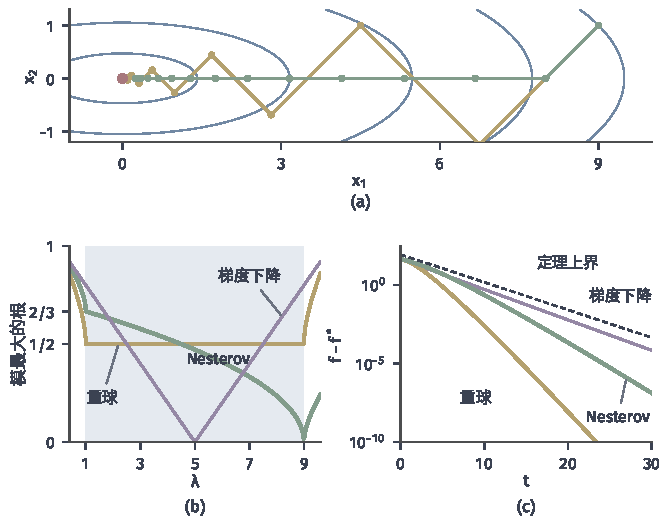
\includegraphics[width=112mm]{figures/05-optimization/02-smooth-optimization/matplotlib/fom-nag-paths/figure.pdf}
  \caption{贯穿例上的Nesterov方法（绿色，$\alpha=1/9$，$\beta=1/2$），对照重球法（黄色，$\alpha=\beta=1/4$）和梯度下降（紫色，$\alpha=1/5$）。(a)等高线上的前$14$步。(b)模最大的根关于$\lambda$的变化，蓝底区间是$[\mu,L]$。(c)目标差，黑色虚线是式~\eqref{eq:fom-nag-strong}给出的上界$86(2/3)^t$。}
  \label{fig:fom-nag-paths}
\end{BookInlineFigure}

要在一般目标上证明收敛，不能再用特征分解，也不能指望函数值单调下降：动量可能把函数值暂时抬高。需要另找一个每步都下降的量，称为\term{势函数}（potential function）。它把“函数值的差”和“某个辅助点到解的距离”加起来，走动时一项增大可以由另一项吸收。

设$q=1/\sqrt\kappa=\sqrt{\mu/L}$，引入辅助点序列$\bm{v}^{(0)}=\bm{x}^{(0)}$，
\begin{equation}
 \bm{v}^{(t+1)}=\bm{x}^{(t)}+\frac1q\bigl(\bm{x}^{(t+1)}-\bm{x}^{(t)}\bigr).
 \label{eq:fom-nag-v}
\end{equation}
它是沿本步位移放大$1/q$倍得到的“更大胆的点”。

\begin{theorem}[强凸情形的Nesterov方法]
\label{thm:fom-nag-strong}
设$f$的梯度$L$-Lipschitz连续且$\mu$强凸，$\mu>0$。取$\alpha=1/L$和式~\eqref{eq:fom-nag-beta-strong}的常数$\beta$，$\bm{x}^{(-1)}=\bm{x}^{(0)}$。则势函数
\begin{equation}
 \Phi^{(t)}=f(\bm{x}^{(t)})-f^\star+\frac\mu2\lVert\bm{v}^{(t)}-\bm{x}^\star\rVert_2^2
 \label{eq:fom-nag-potential}
\end{equation}
满足$\Phi^{(t+1)}\leq(1-1/\sqrt\kappa)\Phi^{(t)}$，因此
\begin{equation}
 f(\bm{x}^{(T)})-f^\star\leq\Bigl(1-\frac{1}{\sqrt\kappa}\Bigr)^T\Bigl(f(\bm{x}^{(0)})-f^\star+\frac\mu2\lVert\bm{x}^{(0)}-\bm{x}^\star\rVert_2^2\Bigr).
 \label{eq:fom-nag-strong}
\end{equation}
\end{theorem}

\begin{proof}
固定一步，省略上标$(t)$，记$\bm{g}=\nabla f(\bm{y})$，$\bm{x}^+$和$\bm{v}^+$为下一步的点。先把辅助点写成便于计算的形式。

第一步，验证两个恒等式：
\[
 \bm{y}=\frac{\bm{x}+q\bm{v}}{1+q},\qquad
 \bm{v}^+=(1-q)\bm{v}+q\bm{y}-\frac q\mu\bm{g}.
\]

第一式在$t=0$时成立。设它对$t$成立，则$q\bm{v}=(1+q)\bm{y}-\bm{x}$，代入第二式右端，并用$\frac{q}{\mu}=\frac{1}{qL}$和$\bm{x}^+=\bm{y}-\bm{g}/L$，化简得到
\[
 \frac1q\bigl(\bm{x}^+-(1-q)\bm{x}\bigr)=\bm{x}+\frac1q(\bm{x}^+-\bm{x}),
\]
正是式~\eqref{eq:fom-nag-v}。再把$\bm{v}^+$代入$(\bm{x}^++q\bm{v}^+)/(1+q)$，得到
\[
 \bm{x}^++\frac{1-q}{1+q}(\bm{x}^+-\bm{x})=\bm{y}^{(t+1)},
\]
所以第一式对$t+1$成立；这里用到$\beta=(1-q)/(1+q)$，它就是式~\eqref{eq:fom-nag-beta-strong}。

第二步，估计距离项。记$\bm{w}=(1-q)\bm{v}+q\bm{y}$，则$\bm{v}^+=\bm{w}-\frac q\mu\bm{g}$，展开平方并乘$\frac\mu2$：
\[
 \frac\mu2\lVert\bm{v}^+-\bm{x}^\star\rVert_2^2
 =\frac\mu2\lVert\bm{w}-\bm{x}^\star\rVert_2^2-q\bm{g}^\top(\bm{w}-\bm{x}^\star)+\frac{q^2}{2\mu}\lVert\bm{g}\rVert_2^2.
\]

第三步，函数项。由下降引理，外推点走一步满足
\[
 f(\bm{x}^+)\leq f(\bm{y})-\frac{1}{2L}\lVert\bm{g}\rVert_2^2.
\]

又$q^2/(2\mu)=1/(2L)$，两边的$\lVert\bm{g}\rVert_2^2$恰好抵消。再用平方范数的凸性拆开$\bm{w}$，得到
\[
 \Phi^{(t+1)}\leq f(\bm{y})-f^\star+(1-q)\frac\mu2\lVert\bm{v}-\bm{x}^\star\rVert_2^2+q\frac\mu2\lVert\bm{y}-\bm{x}^\star\rVert_2^2-q\bm{g}^\top(\bm{w}-\bm{x}^\star).
\]

第四步，处理内积。把$\bm{w}-\bm{x}^\star$拆开：
\[
 \bm{w}-\bm{x}^\star=(1-q)(\bm{v}-\bm{y})+(\bm{y}-\bm{x}^\star).
\]

对后一部分用强凸性：
\[
 q\bm{g}^\top(\bm{y}-\bm{x}^\star)\geq q\bigl(f(\bm{y})-f^\star\bigr)+q\frac\mu2\lVert\bm{y}-\bm{x}^\star\rVert_2^2.
\]
代入后，$\lVert\bm{y}-\bm{x}^\star\rVert_2^2$项抵消，留下
\[
 \Phi^{(t+1)}\leq(1-q)\bigl(f(\bm{y})-f^\star\bigr)+(1-q)\frac\mu2\lVert\bm{v}-\bm{x}^\star\rVert_2^2-q(1-q)\bm{g}^\top(\bm{v}-\bm{y}).
\]

第五步，由第一式$q(\bm{v}-\bm{y})=\bm{y}-\bm{x}$，末项等于$(1-q)\bm{g}^\top(\bm{x}-\bm{y})$。凸性给出
\[
 \bm{g}^\top(\bm{x}-\bm{y})\leq f(\bm{x})-f(\bm{y}),
\]
于是$f(\bm{y})$消去，
\[
 \Phi^{(t+1)}\leq(1-q)\Bigl(f(\bm{x})-f^\star+\frac\mu2\lVert\bm{v}-\bm{x}^\star\rVert_2^2\Bigr)=(1-q)\Phi^{(t)}.
\]

由$\bm{v}^{(0)}=\bm{x}^{(0)}$，迭代得
\[
 f(\bm{x}^{(T)})-f^\star\leq\Phi^{(T)}\leq(1-q)^T\Phi^{(0)}.
\]
\end{proof}

用贯穿例核对势函数。$\mu=1$，$q=\tfrac13$，辅助点由式~\eqref{eq:fom-nag-v}算出，三个势函数值依次是
\[
 \begin{aligned}
 \bm{v}^{(0)}&=(9,1), &\Phi^{(0)}&=45+41=86,\\
 \bm{v}^{(1)}&=(6,-2), &\Phi^{(1)}&=32+20=52,\\
 \bm{v}^{(2)}&=(4,0), &\Phi^{(2)}&\approx22.22+8=30.22.
 \end{aligned}
\]
定理要求每步至少缩小到$\tfrac23$：$86\cdot\tfrac23\approx57.3\geq52$，$52\cdot\tfrac23\approx34.7\geq30.22$。

强凸性给出距离项不超过初始目标差，所以式~\eqref{eq:fom-nag-strong}右端不超过初始目标差的$2(1-1/\sqrt\kappa)^T$倍。所以达到目标差$\varepsilon$的步数约为$\sqrt\kappa\ln(1/\varepsilon)$，与重球法在二次目标上的量级相同，但条件只要求一般的强凸光滑。式~\eqref{eq:fom-hb-counterexample}满足这些条件，定理保证了图~\ref{fig:fom-hb-cycle}中绿线的收敛。

\paragraph{光滑凸情形的势函数分析}
没有强凸常数时，常数的$\beta$无从定义。这时让外推系数随步数增长。定义
\begin{equation}
 \theta^{(0)}=1,\qquad\theta^{(t+1)}=\frac{1+\sqrt{1+4(\theta^{(t)})^2}}{2},\qquad
 \beta^{(t+1)}=\frac{\theta^{(t)}-1}{\theta^{(t+1)}},
 \label{eq:fom-nag-theta}
\end{equation}
并取$\beta^{(0)}=0$，$\alpha=1/L$。$\theta^{(t+1)}$是方程$\theta^2-\theta=(\theta^{(t)})^2$的正根，这个关系在证明中恰好让相邻两项抵消。由$\theta^{(t+1)}\geq\theta^{(t)}+\tfrac12$得$\theta^{(t)}\geq(t+2)/2$，系数$\beta^{(t)}$逐步趋近于$1$。

\begin{theorem}[光滑凸情形的Nesterov方法]
\label{thm:fom-nag-convex}
设$f$凸，梯度$L$-Lipschitz连续，存在最优解$\bm{x}^\star$。按式~\eqref{eq:fom-nag}、\eqref{eq:fom-nag-theta}迭代，$\alpha=1/L$，则对任意$T\geq1$，
\begin{equation}
 f(\bm{x}^{(T)})-f^\star\leq\frac{2L\lVert\bm{x}^{(0)}-\bm{x}^\star\rVert_2^2}{(T+1)^2}.
 \label{eq:fom-nag-convex}
\end{equation}
\end{theorem}

\begin{proof}
第一步，建立一个单步不等式。设$\bm{y}$任意，$\bm{x}^+=\bm{y}-\nabla f(\bm{y})/L$，$\bm{z}$任意。由下降引理和凸性，
\[
 f(\bm{x}^+)\leq f(\bm{z})+\nabla f(\bm{y})^\top(\bm{y}-\bm{z})-\frac{1}{2L}\lVert\nabla f(\bm{y})\rVert_2^2.
\]

把$\nabla f(\bm{y})=L(\bm{y}-\bm{x}^+)$代入，并用恒等式
\[
 2\bm{a}^\top\bm{b}-\lVert\bm{a}\rVert_2^2=\lVert\bm{b}\rVert_2^2-\lVert\bm{b}-\bm{a}\rVert_2^2,
\]
其中$\bm{a}=\bm{y}-\bm{x}^+$，$\bm{b}=\bm{y}-\bm{z}$，得到
\begin{equation}
 f(\bm{x}^+)-f(\bm{z})\leq\frac L2\Bigl(\lVert\bm{y}-\bm{z}\rVert_2^2-\lVert\bm{x}^+-\bm{z}\rVert_2^2\Bigr).
 \label{eq:fom-nag-one-step}
\end{equation}

第二步，选择比较点。省略上标$(t)$，记$\theta=\theta^{(t)}$，$\Delta_t=f(\bm{x}^{(t)})-f^\star$。取
\[
 \bm{z}=\Bigl(1-\frac1\theta\Bigr)\bm{x}+\frac1\theta\bm{x}^\star.
\]

由凸性，
\[
 f(\bm{z})-f^\star\leq\Bigl(1-\frac1\theta\Bigr)\Delta_t.
\]

代入式~\eqref{eq:fom-nag-one-step}，两边乘以$\theta^2$，把$\theta$乘进范数：
\[
 \theta^2\Delta_{t+1}-(\theta^2-\theta)\Delta_t\leq\frac L2\Bigl(\lVert\theta\bm{y}-\theta\bm{z}\rVert_2^2-\lVert\theta\bm{x}^+-\theta\bm{z}\rVert_2^2\Bigr).
\]

第三步，识别辅助点。令
\[
 \bm{v}^{(t)}=\theta^{(t)}\bm{y}^{(t)}-\bigl(\theta^{(t)}-1\bigr)\bm{x}^{(t)},
\]
于是
\[
 \theta\bm{y}-\theta\bm{z}=\bm{v}^{(t)}-\bm{x}^\star.
\]

而由式~\eqref{eq:fom-nag}和式~\eqref{eq:fom-nag-theta}，$\theta^{(t+1)}\bm{y}^{(t+1)}$可以写开，得到
\[
 \bm{v}^{(t+1)}=\bm{x}^{(t)}+\theta^{(t)}\bigl(\bm{x}^{(t+1)}-\bm{x}^{(t)}\bigr),
\]
这恰好是$\theta\bm{x}^+-\theta\bm{z}+\bm{x}^\star$。

第四步，定义势函数$E^{(t)}$并裂项。规定$\theta^{(-1)}=0$，令
\[
 E^{(t)}=\bigl(\theta^{(t-1)}\bigr)^2\Delta_t+\frac L2\lVert\bm{v}^{(t)}-\bm{x}^\star\rVert_2^2.
\]

由$\theta^2-\theta=(\theta^{(t-1)})^2$（$t=0$时两边都是零），上一步的不等式就是$E^{(t+1)}\leq E^{(t)}$。又$\bm{v}^{(0)}=\bm{x}^{(0)}$，所以
\[
 \bigl(\theta^{(T-1)}\bigr)^2\Delta_T\leq E^{(T)}\leq E^{(0)}=\frac L2\lVert\bm{x}^{(0)}-\bm{x}^\star\rVert_2^2.
\]

再用$\theta^{(T-1)}\geq(T+1)/2$，即得式~\eqref{eq:fom-nag-convex}。
\end{proof}

$1/T$变成了$1/T^2$。目标差要达到$\varepsilon$，步数从$LR^2/(2\varepsilon)$降到约$\sqrt{2L/\varepsilon}\,R$。图~\ref{fig:fom-nag-convex}(a)用一个三对角的二次函数验证这一点，它的特征值一路逼近零，强凸常数实际上帮不上忙。

\begin{BookInlineFigure}
  \centering
  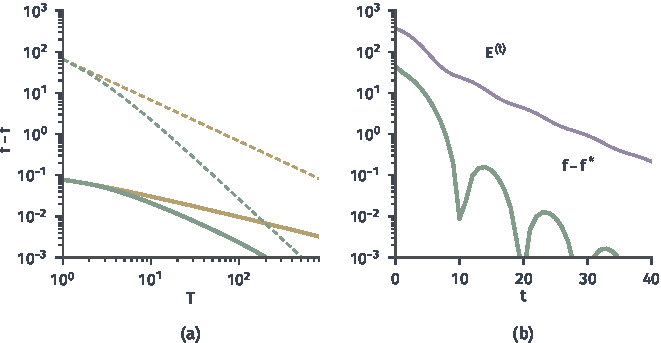
\includegraphics[width=112mm]{figures/05-optimization/02-smooth-optimization/matplotlib/fom-nag-convex/figure.pdf}
  \caption{光滑凸目标上的$1/T$与$1/T^2$。(a)$f(\bm{x})=\tfrac14(\tfrac12\bm{x}^\top\bm{A}\bm{x}-x_1)$，$\bm{A}$是$400$阶三对角矩阵（对角元$2$，次对角元$-1$），$L=1$，$\bm{x}^{(0)}=\bm{0}$。黄线是梯度下降，绿线是Nesterov方法（$\theta$形式），同色虚线是式~\eqref{eq:fom-gd-convex}、\eqref{eq:fom-nag-convex}的上界。(b)贯穿例按$\theta$形式运行，$L=9$：绿线是目标差，出现回升；紫线是势函数$E^{(t)}$，逐步下降。}
  \label{fig:fom-nag-convex}
\end{BookInlineFigure}

图~\ref{fig:fom-nag-convex}(b)说明势函数的用意。贯穿例按式~\eqref{eq:fom-nag-theta}的参数运行时，$\beta^{(t)}$逐渐接近$1$，动量过大，目标差出现$13$次回升，而$E^{(t)}$从$369$（$t=0$）、$320$（$t=1$）一路下降。凸情形的结论控制的是最后一步的目标差上界，并没有说目标差单调下降。

可以用势函数检查第一步的计算：由$\theta^{(0)}=1$得$\bm{v}^{(1)}=\bm{x}^{(1)}=(8,0)$，所以
\[
 E^{(1)}=1\cdot32+\frac92\cdot64=320,\qquad E^{(0)}=\frac92\cdot82=369.
\]

下表把两种动量方法放在一起对比。

\begin{BookInlineTable}
  \centering
  \caption{重球法与Nesterov方法的对比。}
  \label{tab:fom-momentum-compare}
  \begin{tabular}{lll}
   \toprule
   & 重球法 & Nesterov方法\\
   \midrule
   梯度位置 & 当前点$\bm{x}^{(t)}$ & 外推点$\bm{y}^{(t)}$\\
   动量对各方向 & 系数$\beta$相同 & 被$1-\alpha\lambda$压低\\
   $\alpha$ & $4/(\sqrt L+\sqrt\mu)^2$ & $1/L$\\
   强凸时$\beta$ & $\bigl(\frac{\sqrt\kappa-1}{\sqrt\kappa+1}\bigr)^2$ & $\frac{\sqrt\kappa-1}{\sqrt\kappa+1}$\\
   二次目标的速度 & $\frac{\sqrt\kappa-1}{\sqrt\kappa+1}$ & $1-1/\sqrt\kappa$\\
   一般强凸光滑 & 这组参数可能不收敛 & 定理~\ref{thm:fom-nag-strong}\\
   光滑凸 & 本章不给结论 & 定理~\ref{thm:fom-nag-convex}\\
   \bottomrule
  \end{tabular}
\end{BookInlineTable}

\paragraph{适用范围}
两条定理的证明都用切平面比较外推点与当前点、外推点与最优解，这正是凸性的作用。目标非凸时，切平面不再从下方托住目标，势函数的下降论证在第一步就不成立，这两条定理不能直接移用。非凸情形需要带函数值检查或重启的修改版本，另有专门的分析，得到的是驻点型的保证，本章不把上面的结论推广过去。

\section{非线性共轭梯度法}
\label{sec:fom-ncg}

上一节用历史位移修正步子，参数要事先知道$L$，有时还要知道$\mu$。本节换一种用历史的方式：每轮保留上一轮的搜索方向，把它与新梯度组合成新方向，步长由线搜索决定，不需要预先知道曲率常数。要解决的问题是：怎样组合才合理，这样组合之后还能保证什么？

先回到正定二次目标
\[
 f(\bm{x})=\frac12\bm{x}^\top\bm{H}\bm{x}-\bm{b}^\top\bm{x}.
\]

这里已经有一个答案：共轭梯度法。它的梯度$\bm{g}=\bm{H}\bm{x}-\bm{b}$就是残差的相反数，迭代为
\[
 \bm{d}^{(t)}=-\bm{g}^{(t)}+\beta^{(t)}\bm{d}^{(t-1)},\qquad
 \beta^{(t)}=\frac{\lVert\bm{g}^{(t)}\rVert_2^2}{\lVert\bm{g}^{(t-1)}\rVert_2^2},
\]
步长是沿$\bm{d}^{(t)}$的精确最小点。各方向两两关于$\bm{H}$共轭，精确算术下至多$n$步得到解。这些结论的推导可参考\BookChapterRef{chap:krylov-methods}{卷二第15章“Krylov子空间法”}。

共轭的意思是$(\bm{d}^{(i)})^\top\bm{H}\bm{d}^{(j)}=0$。用椭圆的语言说：把椭圆拉成圆后，这些方向互相垂直，所以沿一个方向走到位之后，后面的方向不会破坏已经完成的进度。图~\ref{fig:fom-sd-vs-cg}是贯穿例上的情形：最速下降在折返，共轭梯度第二步直接指向中心。

\begin{BookInlineFigure}
  \centering
  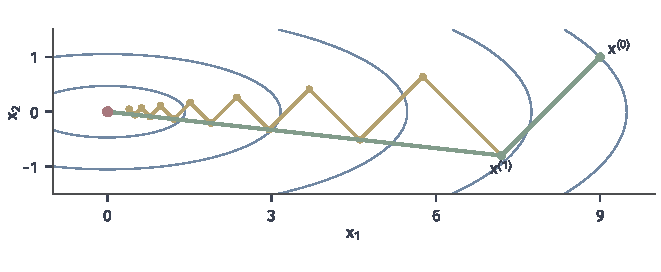
\includegraphics[width=112mm]{figures/05-optimization/02-smooth-optimization/matplotlib/fom-sd-vs-cg/figure.pdf}
  \caption{贯穿例上的精确线搜索路径，蓝色椭圆是等高线。黄色路径是最速下降，绿色路径是共轭梯度法。两者第一步相同，都到达$\bm{x}^{(1)}=(7.2,-0.8)$；共轭梯度的第二步到达最优解（红点），最速下降则继续折返。}
  \label{fig:fom-sd-vs-cg}
\end{BookInlineFigure}

目标不是二次时，两个前提都不存在：没有固定的$\bm{H}$，共轭的定义失去了依托；一般也求不出沿线的精确最小点。\term{非线性共轭梯度法}（nonlinear conjugate gradient method）只保留方向递推的形式，用真实的梯度代替残差，用线搜索代替精确步长。代价是，共轭性一般不再精确保持，有限步终止的结论也不再成立。

\subsection{方向的更新}
\label{sec:fom-ncg-direction}

\paragraph{主要思想}
方法的骨架是
\begin{equation}
 \bm{d}^{(t)}=-\bm{g}^{(t)}+\beta^{(t)}\bm{d}^{(t-1)},\qquad
 \bm{x}^{(t+1)}=\bm{x}^{(t)}+\alpha^{(t)}\bm{d}^{(t)},
 \label{eq:fom-ncg}
\end{equation}
其中$\bm{d}^{(0)}=-\bm{g}^{(0)}$。它只比梯度下降多存一个向量。需要决定的只有两件事：$\beta^{(t)}$怎样算，$\alpha^{(t)}$怎样选。这一小节讨论前者。

在二次目标上，$\beta^{(t)}$可以写成好几种形式，它们彼此相等。写法不同，推广到非线性时就成了不同的算法。从共轭条件出发，要求$(\bm{d}^{(t)})^\top\bm{H}\bm{d}^{(t-1)}=0$，由式~\eqref{eq:fom-ncg}得
\[
 \beta^{(t)}=\frac{(\bm{g}^{(t)})^\top\bm{H}\bm{d}^{(t-1)}}{(\bm{d}^{(t-1)})^\top\bm{H}\bm{d}^{(t-1)}}.
\]

式中含有$\bm{H}$，非线性时无法直接使用。在二次目标上，相邻梯度之差恰好是$\bm{H}$作用在位移上：
\[
 \bm{\delta}^{(t)}:=\bm{g}^{(t)}-\bm{g}^{(t-1)}=\alpha^{(t-1)}\bm{H}\bm{d}^{(t-1)}.
\]

把它代入上式，消去$\alpha^{(t-1)}$，得到只含梯度和方向的表达式：
\[
 \beta^{(t)}=\frac{(\bm{g}^{(t)})^\top\bm{\delta}^{(t)}}{(\bm{d}^{(t-1)})^\top\bm{\delta}^{(t)}}.
\]

精确线搜索使$(\bm{g}^{(t)})^\top\bm{d}^{(t-1)}=0$，并且同样有$(\bm{g}^{(t-1)})^\top\bm{d}^{(t-2)}=0$，由式~\eqref{eq:fom-ncg}得
\[
 (\bm{d}^{(t-1)})^\top\bm{\delta}^{(t)}=-(\bm{d}^{(t-1)})^\top\bm{g}^{(t-1)}=\lVert\bm{g}^{(t-1)}\rVert_2^2.
\]

这样分母化成了$\lVert\bm{g}^{(t-1)}\rVert_2^2$，得到\term{Polak--Ribière--Polyak公式}（Polak--Ribière--Polyak formula，PRP）：
\begin{equation}
 \beta_{\mathrm{PRP}}^{(t)}=\frac{(\bm{g}^{(t)})^\top\bigl(\bm{g}^{(t)}-\bm{g}^{(t-1)}\bigr)}{\lVert\bm{g}^{(t-1)}\rVert_2^2}.
 \label{eq:fom-beta-prp}
\end{equation}

再用线性共轭梯度中相邻梯度的正交性$(\bm{g}^{(t)})^\top\bm{g}^{(t-1)}=0$，分子只剩$\lVert\bm{g}^{(t)}\rVert_2^2$，得到\term{Fletcher--Reeves公式}（Fletcher--Reeves formula，FR）：
\begin{equation}
 \beta_{\mathrm{FR}}^{(t)}=\frac{\lVert\bm{g}^{(t)}\rVert_2^2}{\lVert\bm{g}^{(t-1)}\rVert_2^2}.
 \label{eq:fom-beta-fr}
\end{equation}

两个公式利用的信息不同。FR只看两个梯度的长度，恒为正；PRP还看梯度变化$\bm{\delta}^{(t)}$，它含有两点之间的曲率信息，符号可正可负。在正定二次目标加精确线搜索时两者一致，离开这个条件就是两个算法，下降性和收敛性要分别讨论。

\needspace{6\baselineskip}
\paragraph{变量}
\begin{itemize}
 \item $\bm{x}^{(t)}\in\mathbb{R}^n$：当前点。
 \item $\bm{g}^{(t)},\bm{g}^{(t-1)}\in\mathbb{R}^n$：当前与上一轮的梯度，FR只需要它们的长度平方，PRP需要向量。
 \item $\bm{d}^{(t)}\in\mathbb{R}^n$：搜索方向，算出新方向后覆盖。
 \item $\alpha^{(t)}$，$\beta^{(t)}$：步长与组合系数，用后即弃。
 \item $\varepsilon$，$T$：容差与最大步数。
\end{itemize}

\paragraph{初始化}
令$\bm{g}^{(0)}=\nabla f(\bm{x}^{(0)})$，$\bm{d}^{(0)}=-\bm{g}^{(0)}$，$t=0$。例中
\[
 \bm{g}^{(0)}=(9,9),\qquad\bm{d}^{(0)}=(-9,-9),\qquad\lVert\bm{g}^{(0)}\rVert_2^2=162.
\]

\needspace{6\baselineskip}
\paragraph{每轮更新}
在第$t$轮：
\begin{enumerate}
 \item \textbf{线搜索。}沿$\bm{d}^{(t)}$确定步长$\alpha^{(t)}$。这里先用精确步长，下一小节讨论实际的规则。二次目标的精确步长是
 \[
  \alpha^{(t)}=-\frac{(\bm{g}^{(t)})^\top\bm{d}^{(t)}}{(\bm{d}^{(t)})^\top\bm{H}\bm{d}^{(t)}}.
 \]
 例中第一轮
 \[
  \alpha^{(0)}=\frac{162}{(-9)^2\cdot1+(-9)^2\cdot9}=\frac{162}{810}=\frac15.
 \]

\item \textbf{更新点并读取新梯度。}由式~\eqref{eq:fom-ncg}得到$\bm{x}^{(t+1)}$，并计算$\bm{g}^{(t+1)}$。例中第一轮
 \[
  \bm{x}^{(1)}=(7.2,-0.8),\qquad\bm{g}^{(1)}=(7.2,-7.2).
 \]

\item \textbf{检查停止。}若$\lVert\bm{g}^{(t+1)}\rVert_2\leq\varepsilon$或已达$T$步，输出$\bm{x}^{(t+1)}$。例中第一轮$\lVert\bm{g}^{(1)}\rVert_2^2=103.68$，继续。

\item \textbf{计算系数并更新方向。}按式~\eqref{eq:fom-beta-fr}或式~\eqref{eq:fom-beta-prp}算$\beta^{(t+1)}$，再由式~\eqref{eq:fom-ncg}算$\bm{d}^{(t+1)}$，令$t\leftarrow t+1$。例中第一轮，$(\bm{g}^{(1)})^\top\bm{g}^{(0)}=0$，所以两个公式给出同一值：
 \[
  \beta^{(1)}=\frac{103.68}{162}=0.64.
 \]
 新方向是
 \[
  \bm{d}^{(1)}=(-7.2,7.2)+0.64(-9,-9)=(-12.96,\,1.44).
 \]
 可以核对共轭关系：
 \[
  (\bm{d}^{(1)})^\top\bm{H}\bm{d}^{(0)}=116.64-116.64=0.
 \]

 例中第二轮线搜索，方向导数和曲率分别是
 \[
  -(\bm{g}^{(1)})^\top\bm{d}^{(1)}=103.68,\qquad(\bm{d}^{(1)})^\top\bm{H}\bm{d}^{(1)}=186.624,
 \]
 于是
 \[
  \alpha^{(1)}=\frac{103.68}{186.624}=\frac59,\qquad
  \bm{x}^{(2)}=(7.2,-0.8)+\tfrac59(-12.96,1.44)=(0,0).
 \]
 此时$\bm{g}^{(2)}=\bm{0}$，满足停止条件。
\end{enumerate}

最终得到$\bm{x}^{(2)}=\bm{x}^\star$。二维的二次目标两步到达，这与$n$步终止的结论相符。图~\ref{fig:fom-ncg-direction}画出第二轮方向的合成：新梯度方向$-\bm{g}^{(1)}$与上一方向$\bm{d}^{(0)}$按平行四边形相加，结果恰好指向椭圆中心。

\begin{BookInlineFigure}
  \centering
  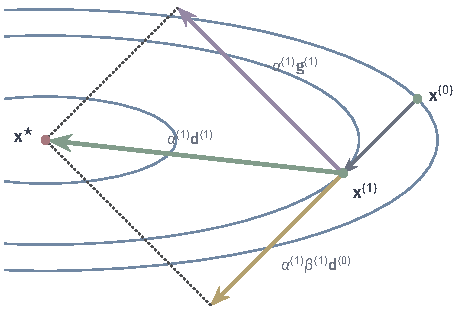
\includegraphics[width=80mm]{figures/05-optimization/02-smooth-optimization/tikz/fom-ncg-direction/figure.pdf}
  \caption{贯穿例第二轮的方向合成，蓝色椭圆是等高线。紫色箭头是负梯度$-\bm{g}^{(1)}$，黄色箭头是上一方向$\bm{d}^{(0)}$乘以$\beta^{(1)}=0.64$，两者都按步长$\alpha^{(1)}=5/9$缩放。绿色箭头是它们的和，从$\bm{x}^{(1)}$直达最优解（红点）。}
  \label{fig:fom-ncg-direction}
\end{BookInlineFigure}

\paragraph{两个公式何时不同}
精确线搜索一旦放宽，即使目标还是二次的，两个公式也立刻分开。在贯穿例第一轮取$\alpha^{(0)}=1/9$，它满足下一小节将列出的线搜索条件，于是
\[
 \bm{x}^{(1)}=(8,0),\qquad\bm{g}^{(1)}=(8,0),\qquad(\bm{g}^{(1)})^\top\bm{g}^{(0)}=72.
\]

这时相邻梯度不再正交。两个系数分别是
\[
 \beta_{\mathrm{FR}}^{(1)}=\frac{64}{162}\approx0.395,\qquad
 \beta_{\mathrm{PRP}}^{(1)}=\frac{64-72}{162}\approx-0.049.
\]

PRP的系数是负的，符号都不同了。对应的方向是
\[
 \bm{d}_{\mathrm{FR}}^{(1)}\approx(-11.56,\,-3.56),\qquad
 \bm{d}_{\mathrm{PRP}}^{(1)}\approx(-7.56,\,0.44).
\]
两者都不再与$\bm{d}^{(0)}$共轭，例如
\[
 (\bm{d}_{\mathrm{FR}}^{(1)})^\top\bm{H}\bm{d}^{(0)}=392\neq0.
\]
方程的形式相同，并不意味着结论相同。

目标非二次时，共轭性的流失更彻底。把贯穿例弯曲一下，取
\begin{equation}
 f(\bm{x})=\frac12x_1^2+\frac92\bigl(x_2-0.1x_1^2\bigr)^2.
 \label{eq:fom-bent}
\end{equation}
这是一条沿抛物线弯曲的山谷，$\bm{x}^\star=\bm{0}$处的Hessian仍是$\operatorname{diag}(1,9)$，系数$0.1$换成零就回到式~\eqref{eq:fom-example}。

图~\ref{fig:fom-ncg-bent}(b)用近乎精确的线搜索运行PRP，并计算相邻方向在当前Hessian下的共轭余弦。它在开始时接近$0.8$，远不是零；直到迭代进入极小点附近、目标接近二次，这个量才逐渐变小。这个二维问题走了$9$步才把梯度降到$10^{-6}$以下，$n$步终止不再成立。

\begin{BookInlineFigure}
  \centering
  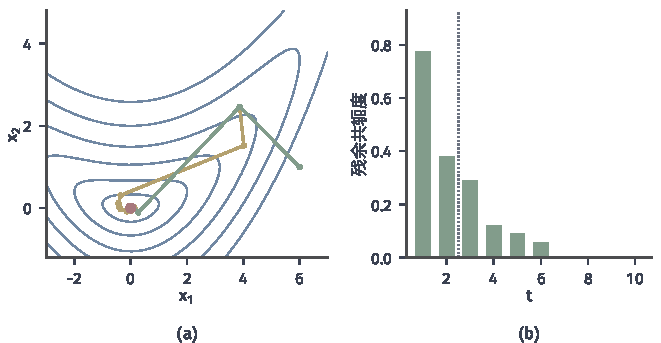
\includegraphics[width=112mm]{figures/05-optimization/02-smooth-optimization/matplotlib/fom-ncg-bent/figure.pdf}
  \caption{弯谷目标~\eqref{eq:fom-bent}上的非线性共轭梯度法，起点$(6,1)$。(a)黄线FR，绿线是把负的PRP系数截断为零的变体PRP+，都采用强Wolfe线搜索（$c_1=10^{-4}$，$c_2=0.4$），画出前$17$步。(b)近似精确线搜索下的PRP，相邻方向的残余共轭度$\lvert(\bm{d}^{(t)})^\top\nabla^2f\,\bm{d}^{(t-1)}\rvert$除以两方向的$\nabla^2f$长度之积，Hessian取在$\bm{x}^{(t)}$；虚线之前是二次目标应该结束的步数。}
  \label{fig:fom-ncg-bent}
\end{BookInlineFigure}

\subsection{线搜索与重启}
\label{sec:fom-ncg-linesearch}

\paragraph{强Wolfe条件}
实际中一般不求沿线精确的最小点。第~\ref{chap:smooth-foundations}章的强Wolfe条件要求步长$\alpha$既满足Armijo条件~\eqref{eq:fom-armijo}，又让方向导数的绝对值变小：
\begin{equation}
 \bigl\lvert\nabla f(\bm{x}+\alpha\bm{d})^\top\bm{d}\bigr\rvert\leq c_2\bigl\lvert\nabla f(\bm{x})^\top\bm{d}\bigr\rvert,\qquad 0<c_1<c_2<1.
 \label{eq:fom-strong-wolfe}
\end{equation}
前一个条件防止走得太远，后一个条件防止走得太近，同时把新点放到沿线函数接近平坦的位置。

贯穿例沿$\bm{d}^{(0)}=(-9,-9)$的一维函数是$\varphi(\alpha)=45-162\alpha+405\alpha^2$，方向导数为$\varphi'(\alpha)=-162+810\alpha$。取$c_1=0.1$，$c_2=0.45$，Armijo条件给出$\alpha\leq0.36$，强Wolfe条件给出
\[
 0.11\leq\alpha\leq0.29.
\]
图~\ref{fig:fom-wolfe}中，$\alpha=1/9$落在区间内，精确步长$1/5$也在区间内。

\begin{BookInlineFigure}
  \centering
  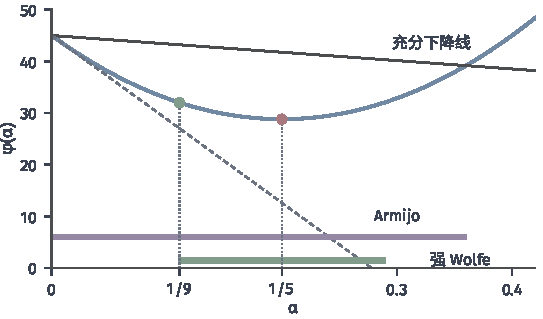
\includegraphics[width=92mm]{figures/05-optimization/02-smooth-optimization/matplotlib/fom-wolfe/figure.pdf}
  \caption{线搜索的可接受区间。蓝色曲线是贯穿例沿$\bm{d}^{(0)}$的$\varphi(\alpha)$，黑色实线是$c_1=0.1$的充分下降线，虚线是$\varphi$在$0$处的切线。紫色线段是Armijo条件接受的区间，绿色线段是再加上$c_2=0.45$的强Wolfe区间。绿点是$\alpha=1/9$，红点是精确最小点$\alpha=1/5$。}
  \label{fig:fom-wolfe}
\end{BookInlineFigure}

\paragraph{FR的下降保证}
方向必须是下降方向，线搜索才有意义。梯度下降中这是自动的，这里却不一定：$(\bm{g}^{(t)})^\top\bm{d}^{(t)}$等于$-\lVert\bm{g}^{(t)}\rVert_2^2$加上$\beta^{(t)}(\bm{g}^{(t)})^\top\bm{d}^{(t-1)}$，后一项可以是正的。精确线搜索让后一项为零；不精确时，强Wolfe条件要限制它的大小。对FR，这需要把$c_2$压到$\tfrac12$以下。

\begin{lemma}[FR方向的下降性]
\label{lem:fom-fr-descent}
设$f$连续可微，每步按强Wolfe条件取$\alpha^{(t)}$，$0<c_1<c_2<\tfrac12$，$\beta^{(t)}$取式~\eqref{eq:fom-beta-fr}，且$\bm{g}^{(t)}\neq\bm{0}$。则对所有$t$，
\begin{equation}
 -\frac{1}{1-c_2}\leq\frac{(\bm{g}^{(t)})^\top\bm{d}^{(t)}}{\lVert\bm{g}^{(t)}\rVert_2^2}\leq\frac{2c_2-1}{1-c_2}<0.
 \label{eq:fom-fr-descent}
\end{equation}
\end{lemma}

\begin{proof}
记中间的比值为$\tau^{(t)}$。对$t$归纳。$t=0$时$\tau^{(0)}=-1$，而
\[
 -\frac{1}{1-c_2}\leq-1\leq\frac{2c_2-1}{1-c_2},
\]
后一个不等号等价于$c_2\geq0$。

设结论对$t$成立，特别地$\bm{d}^{(t)}$是下降方向，线搜索可以进行。由式~\eqref{eq:fom-ncg}和$\beta_{\mathrm{FR}}^{(t+1)}$的定义，
\[
 \tau^{(t+1)}=-1+\frac{(\bm{g}^{(t+1)})^\top\bm{d}^{(t)}}{\lVert\bm{g}^{(t)}\rVert_2^2}.
\]

强Wolfe条件~\eqref{eq:fom-strong-wolfe}给出
\[
 \bigl\lvert(\bm{g}^{(t+1)})^\top\bm{d}^{(t)}\bigr\rvert\leq-c_2(\bm{g}^{(t)})^\top\bm{d}^{(t)}.
\]

除以$\lVert\bm{g}^{(t)}\rVert_2^2$，得到
\[
 -1+c_2\tau^{(t)}\leq\tau^{(t+1)}\leq-1-c_2\tau^{(t)}.
\]

代入归纳假设的下界$\tau^{(t)}\geq-1/(1-c_2)$，左端不小于$-1/(1-c_2)$，右端不大于$(2c_2-1)/(1-c_2)$。由$c_2<\tfrac12$，右端为负。
\end{proof}

用上面$\alpha^{(0)}=1/9$的数据检验。$c_2=0.45$时$\alpha^{(0)}$可接受，引理的区间是$[-1.82,-0.18]$，而
\[
 \tau^{(1)}=\frac{(8,0)^\top(-11.56,-3.56)}{64}\approx-1.44,
\]
确实落在区间内。

\paragraph{FR的全局收敛}
下降方向还不够，还要防止方向几乎与梯度垂直。记$\theta^{(t)}$为$\bm{d}^{(t)}$与$-\bm{g}^{(t)}$的夹角。Wolfe条件带来一个累加估计，它把线搜索的效果转化为对夹角的约束。

\begin{lemma}[Zoutendijk条件]
\label{lem:fom-zoutendijk}
设$f$有下界，梯度$L$-Lipschitz连续，$\bm{d}^{(t)}$都是下降方向，步长满足Armijo条件和Wolfe曲率条件（方向导数至少升到原值的$c_2$倍，$0<c_1<c_2<1$）。则
\begin{equation}
 \sum_{t=0}^\infty\cos^2\theta^{(t)}\lVert\bm{g}^{(t)}\rVert_2^2<\infty.
 \label{eq:fom-zoutendijk}
\end{equation}
\end{lemma}

\begin{proof}
曲率条件是
\[
 (\bm{g}^{(t+1)})^\top\bm{d}^{(t)}\geq c_2(\bm{g}^{(t)})^\top\bm{d}^{(t)}.
\]

两边减去$(\bm{g}^{(t)})^\top\bm{d}^{(t)}$，得到
\[
 (\bm{g}^{(t+1)}-\bm{g}^{(t)})^\top\bm{d}^{(t)}\geq(c_2-1)(\bm{g}^{(t)})^\top\bm{d}^{(t)}.
\]

由梯度Lipschitz，左端不超过$\alpha^{(t)}L\lVert\bm{d}^{(t)}\rVert_2^2$。于是步长有下界
\[
 \alpha^{(t)}\geq\frac{(1-c_2)\lvert(\bm{g}^{(t)})^\top\bm{d}^{(t)}\rvert}{L\lVert\bm{d}^{(t)}\rVert_2^2}.
\]

代入Armijo条件，并用$\lvert\bm{g}^\top\bm{d}\rvert$与$\cos\theta$的关系，得到
\[
 f(\bm{x}^{(t)})-f(\bm{x}^{(t+1)})\geq\frac{c_1(1-c_2)}{L}\cos^2\theta^{(t)}\lVert\bm{g}^{(t)}\rVert_2^2.
\]

对$t$求和，函数值裂项，再用下界，即得结论。
\end{proof}

\begin{theorem}[FR与强Wolfe线搜索]
\label{thm:fom-fr-convergence}
设$f$有下界，梯度$L$-Lipschitz连续。按FR公式迭代，步长满足强Wolfe条件，$0<c_1<c_2<\tfrac12$。若每步$\bm{g}^{(t)}\neq\bm{0}$，则
\begin{equation}
 \liminf_{t\to\infty}\lVert\bm{g}^{(t)}\rVert_2=0.
 \label{eq:fom-fr-convergence}
\end{equation}
\end{theorem}

\begin{proof}
用反证法。设存在$\gamma>0$使$\lVert\bm{g}^{(t)}\rVert_2\geq\gamma$对所有$t$成立。先估计方向的长度。由引理~\ref{lem:fom-fr-descent}，
\[
 \bigl\lvert(\bm{g}^{(t)})^\top\bm{d}^{(t)}\bigr\rvert\leq\frac{\lVert\bm{g}^{(t)}\rVert_2^2}{1-c_2}.
\]

再由强Wolfe条件，并用FR公式把$\beta^{(t+1)}\lVert\bm{g}^{(t)}\rVert_2^2$换成$\lVert\bm{g}^{(t+1)}\rVert_2^2$，展开$\lVert\bm{d}^{(t+1)}\rVert_2^2$，得到
\[
 \lVert\bm{d}^{(t+1)}\rVert_2^2\leq\frac{1+c_2}{1-c_2}\lVert\bm{g}^{(t+1)}\rVert_2^2+\bigl(\beta^{(t+1)}\bigr)^2\lVert\bm{d}^{(t)}\rVert_2^2.
\]

记$c=(1+c_2)/(1-c_2)\geq1$。两边除以$\lVert\bm{g}^{(t+1)}\rVert_2^4$，由FR公式消去$\beta^{(t+1)}$，因此
\[
 \frac{\lVert\bm{d}^{(t+1)}\rVert_2^2}{\lVert\bm{g}^{(t+1)}\rVert_2^4}\leq\frac{\lVert\bm{d}^{(t)}\rVert_2^2}{\lVert\bm{g}^{(t)}\rVert_2^4}+\frac{c}{\lVert\bm{g}^{(t+1)}\rVert_2^2}.
\]

由$\bm{d}^{(0)}=-\bm{g}^{(0)}$，归纳可得
\[
 \frac{\lVert\bm{d}^{(t)}\rVert_2^2}{\lVert\bm{g}^{(t)}\rVert_2^4}\leq\frac{c(t+1)}{\gamma^2}.
\]

再由引理~\ref{lem:fom-fr-descent}的上界，
\[
 \lvert\bm{g}^\top\bm{d}\rvert\geq c'\lVert\bm{g}\rVert_2^2,\qquad c'=\frac{1-2c_2}{1-c_2}>0.
\]
所以
\[
 \cos^2\theta^{(t)}\lVert\bm{g}^{(t)}\rVert_2^2=\frac{(\bm{g}^\top\bm{d})^2}{\lVert\bm{d}\rVert_2^2}\geq\frac{c'^2\lVert\bm{g}\rVert_2^4}{\lVert\bm{d}\rVert_2^2}\geq\frac{c'^2\gamma^2}{c(t+1)}.
\]

右端对$t$求和发散，与式~\eqref{eq:fom-zoutendijk}矛盾。
\end{proof}

定理不要求凸，结论是驻点型的，而且只是$\liminf$，说明有一列子序列的梯度趋于零。它与定理~\ref{thm:fom-gd-nonconvex}的$\lVert\bm{g}^{(t)}\rVert_2\to0$相比更弱，也不给出步数的界。

条件$c_2<\tfrac12$在这里是起作用的：引理的证明里，它让上界保持为负。一旦$c_2\geq\tfrac12$，上述论证不能保证方向下降。

\paragraph{FR的卡顿与PRP的自动重启}
定理保证了极限，却不保证速度。FR有一种典型的卡顿现象。若某一步步长很小，$\bm{g}^{(t)}\approx\bm{g}^{(t-1)}$，那么$\beta_{\mathrm{FR}}^{(t)}\approx1$，新方向约为$-\bm{g}^{(t)}+\bm{d}^{(t-1)}$，几乎沿用了旧方向。旧方向已经效果不佳，下一步又只能走很小的一步，如此延续。

PRP在同样的情形下，分子含有接近零的差$\bm{g}^{(t)}-\bm{g}^{(t-1)}$，于是$\beta_{\mathrm{PRP}}^{(t)}\approx0$，方向自动回到负梯度，相当于重新开始。这就是实践中PRP一般比FR好的原因。图~\ref{fig:fom-ncg-restart}在弯谷上对比了它们。

\begin{BookInlineFigure}
  \centering
  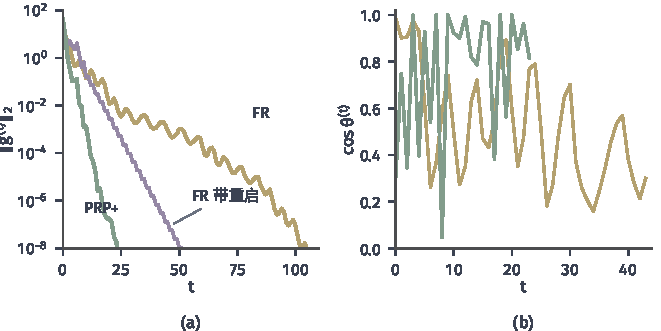
\includegraphics[width=112mm]{figures/05-optimization/02-smooth-optimization/matplotlib/fom-ncg-restart/figure.pdf}
  \caption{弯谷目标~\eqref{eq:fom-bent}上的三种方案，起点$(6,1)$，强Wolfe线搜索$c_1=10^{-4}$，$c_2=0.4$。(a)梯度大小：黄线是FR，紫线是FR加Powell重启（式~\eqref{eq:fom-powell-restart}，$\nu=0.1$），绿线是PRP+。(b)$\bm{d}^{(t)}$与$-\bm{g}^{(t)}$的夹角余弦：黄线FR在后期长时间偏低，绿线PRP+能够多次回到接近$1$的位置。}
  \label{fig:fom-ncg-restart}
\end{BookInlineFigure}

\paragraph{PRP+的下降保障}
PRP的优点有代价。Powell构造过非凸的例子，PRP配合精确线搜索也可能在一组非驻点之间循环，这说明全局收敛不能指望公式本身。这样的反例需要专门构造，证明的细节读者可查阅\scite{math-nocedal2006numerical}。

一个常用的修改是把负的系数截断为零：
\begin{equation}
 \beta_{\mathrm{PRP+}}^{(t)}=\max\bigl\{\beta_{\mathrm{PRP}}^{(t)},\,0\bigr\}.
 \label{eq:fom-beta-prp-plus}
\end{equation}
其含义是：若梯度变化表明上一方向已不再有帮助，就直接扔掉它。贯穿例上$\alpha^{(0)}=1/9$的那一步，PRP+的$\beta$就是$0$，新方向是负梯度$(-8,0)$。

只截断还不够。与FR不同，PRP+在强Wolfe条件下并不自动产生下降方向，因为$\beta$的大小不再受$\lVert\bm{g}^{(t)}\rVert_2^2/\lVert\bm{g}^{(t-1)}\rVert_2^2$限制。已知的收敛定理要求额外的条件：$f$的下水平集有界，梯度Lipschitz，线搜索除强Wolfe条件之外还要保证充分下降，即存在$c>0$使
\begin{equation}
 (\bm{g}^{(t)})^\top\bm{d}^{(t)}\leq-c\lVert\bm{g}^{(t)}\rVert_2^2.
 \label{eq:fom-sufficient-descent}
\end{equation}
在这些条件下可以得到$\liminf\lVert\bm{g}^{(t)}\rVert_2=0$。证明要追踪归一化方向的变化量并作累计估计，篇幅较长，读者可查阅\scite{math-nocedal2006numerical}。这个结论本章没有证明，它依赖的是“PRP+、线搜索与充分下降”三者的组合，缺一项就不能引用。

\paragraph{重启}
非线性情形下，旧方向携带的曲率信息随着地形变化而过期。\term{重启}（restart）就是把方向重置为负梯度，丢弃旧方向。常用的触发条件有三种。

第一种检测方向不再下降：若新方向不满足式~\eqref{eq:fom-sufficient-descent}，立即令$\bm{d}^{(t)}=-\bm{g}^{(t)}$。第二种按周期：每$n$步重启一次，相当于让方向序列按段重新建立。第三种由Powell提出，检测相邻梯度偏离了线性共轭梯度中的正交性：若
\begin{equation}
 \bigl\lvert(\bm{g}^{(t)})^\top\bm{g}^{(t-1)}\bigr\rvert\geq\nu\lVert\bm{g}^{(t)}\rVert_2^2,\qquad\nu\approx0.1,
 \label{eq:fom-powell-restart}
\end{equation}
就重启。

重启并不总是有益的。图~\ref{fig:fom-ncg-restart}(a)的数据是：从$(6,1)$出发，目标梯度$10^{-8}$，FR走了$105$步，加上重启后降到$52$步，PRP+只要$24$步。而对PRP+再加上式~\eqref{eq:fom-powell-restart}，在贯穿起点$(9,1)$上反而从$28$步增加到$52$步，因为PRP+本身已经在需要时自动重置，额外的重启浪费了仍然有用的方向。

下表把变体、线搜索和保证的组合列在一起。引用某个结论时，三列必须同时对应。

\begin{BookInlineTable}
  \centering
  \caption{非线性共轭梯度的常见组合，表中收敛都是$\liminf\lVert\bm{g}^{(t)}\rVert_2=0$。}
  \label{tab:fom-ncg-combos}
  \begin{tabular}{lll}
   \toprule
   变体 & 线搜索与附加条件 & 下降性与收敛\\
   \midrule
   FR & 强Wolfe，$c_2<\tfrac12$ & 下降，定理~\ref{thm:fom-fr-convergence}\\
   PRP & 精确或强Wolfe & 可能循环，无一般保证\\
   PRP+ & 强Wolfe，式~\eqref{eq:fom-sufficient-descent} & 收敛，本章未证\\
   加重启 & 依所用变体 & 保证随所用规则核对\\
   \bottomrule
  \end{tabular}
\end{BookInlineTable}

\section{收敛与计算成本}
\label{sec:fom-cost}

前三节各自给出了保证和例子。于是要问：要在几种方法中选择时，应该按什么标准比较？按第~\ref{chap:smooth-foundations}章的约定，比较时要固定三件事：度量误差的量、停止精度和要报告的迭代点，然后计算达到这一精度所需的总计算。

\paragraph{同样的尺子}
贯穿例上，以梯度大小不超过$10^{-3}$为停止标准，各方法的结果如下表。固定步长的方法每步读一次梯度，读取次数与步数大体相等。

\begin{BookInlineTable}
  \centering
  \caption{贯穿例上达到$\lVert\bm{g}\rVert_2\leq10^{-3}$的步数。}
  \label{tab:fom-example-count}
  \begin{tabular}{lll}
   \toprule
   方法 & 参数 & 步数\\
   \midrule
   梯度下降 & $\alpha=1/9$ & $78$\\
   梯度下降 & $\alpha=1/5$ & $43$\\
   重球法 & $\alpha=\beta=1/4$ & $19$\\
   Nesterov方法 & $\alpha=1/9$，$\beta=1/2$ & $29$\\
   共轭梯度 & 精确线搜索 & $2$\\
   \bottomrule
  \end{tabular}
\end{BookInlineTable}

这张表不能拿来宣布胜负。共轭梯度的$2$步依赖于目标是二次的，而且精确步长用到了$\bm{H}$；重球法的$19$步依赖于事先知道$\mu$和$L$，并且只对二次目标有理论保证；三种固定步长的方法都不必做线搜索。下面把这些差异分别计入。

\paragraph{保证的比较}
下表汇总本章的保证，$R=\lVert\bm{x}^{(0)}-\bm{x}^\star\rVert_2$，$\Delta=f(\bm{x}^{(0)})-f_{\inf}$。不同列的度量不同：非凸列是梯度大小，凸与强凸列是目标差。

\begin{BookInlineTable}
  \centering
  \caption{各方法的理论保证，$\Phi^{(0)}=f(\bm{x}^{(0)})-f^\star+\tfrac\mu2R^2$，“—”表示本章不给结论。}
  \label{tab:fom-guarantees}
  \begin{tabular}{llll}
   \toprule
   方法 & 非凸 & 凸 & 强凸\\
   \midrule
   梯度下降 & $\min\lVert\bm{g}\rVert_2^2\leq\frac{2L\Delta}{T}$ & $\frac{LR^2}{2T}$ & $(1-\frac1\kappa)^T\Delta$\\
   重球法 & — & — & 二次目标$(2T+1)\rho^T$\\
   Nesterov方法 & — & $\frac{2LR^2}{(T+1)^2}$ & $(1-\frac{1}{\sqrt\kappa})^T\Phi^{(0)}$\\
   FR & $\liminf\lVert\bm{g}\rVert_2=0$ & 同左 & 同左\\
   \bottomrule
  \end{tabular}
\end{BookInlineTable}

重球法一行的界是解距离的比例，$\rho=(\sqrt\kappa-1)/(\sqrt\kappa+1)$。FR的“同左”表示在凸和强凸情形下，本章的定理仍然只给出驻点型的结论。这与实际的快慢不是一回事：FR在实践中常比梯度下降快，但本章的定理没有给出这一点。

$T$与$\kappa$的影响可以换算成具体的数字。取$\kappa=10^4$，目标差要降到初值的$10^{-6}$，$\ln10^6\approx13.8$，于是
\[
 \kappa\ln\frac1\varepsilon\approx1.38\times10^5,\qquad
 \sqrt\kappa\ln\frac1\varepsilon\approx1.38\times10^3.
\]

相差一百倍。这是梯度下降与加速方法在定理的上界上的差别。Nesterov方法的$\sqrt\kappa$和$1/T^2$依赖，在“新迭代点只在已读取梯度的张成空间内”这类方法中不能进一步改进；证明需要构造一个三对角的二次函数，让前$T$步的梯度只能探到前$T$个坐标，篇幅较长，读者可查阅凸优化的专门著作。图~\ref{fig:fom-nag-convex}所用的函数正是这种构造。

\paragraph{一步要花多少}
迭代次数只是总计算的一个因子。每步的代价由三部分构成：梯度读取、线搜索的函数试探、向量的更新与存储。

\begin{BookInlineTable}
  \centering
  \caption{每步的代价，维数为$n$。}
  \label{tab:fom-cost-per-step}
  \begin{tabular}{llll}
   \toprule
   方法 & 梯度读取 & 存储向量 & 需要的信息\\
   \midrule
   梯度下降（固定） & $1$ & $2$ & $L$\\
   梯度下降（回溯） & $1$加试探 & $2$ & 无\\
   重球法 & $1$ & $3$ & $L,\mu$\\
   Nesterov方法 & $1$ & $3$ & $L$，强凸时加$\mu$\\
   非线性共轭梯度 & 多次 & $3$到$4$ & 无\\
   \bottomrule
  \end{tabular}
\end{BookInlineTable}

向量更新都是$O(n)$，与读一次梯度相比通常可以忽略。除非目标是高度结构化的，读一次梯度的代价要大得多。所以比较的主要量是梯度与函数的读取次数，而不是迭代步数。

强Wolfe线搜索每步要在试探点上计算函数值和方向导数，后者需要整个梯度，一次试探大约相当于一次完整的梯度读取。试探次数取决于初始步长的猜测和$c_2$的松紧。例如弯谷上$c_2=0.4$时，PRP+走了$24$步，用了$75$次读取，平均每步约$3$次。

\paragraph{步数少不等于计算少}
图~\ref{fig:fom-cost}在一个$100$维的问题上比较四种方法：
\[
 f(\bm{x})=\frac12\sum_{i=1}^{100}\lambda_ix_i^2+\sum_{i=1}^{100}\ln\cosh x_i,
\]
其中$\lambda_i$在$[1,1000]$内按对数等距分布。目标强凸，$\mu=1$，$L=1001$，要求$\lVert\bm{g}\rVert_2\leq10^{-6}$。

\begin{BookInlineFigure}
  \centering
  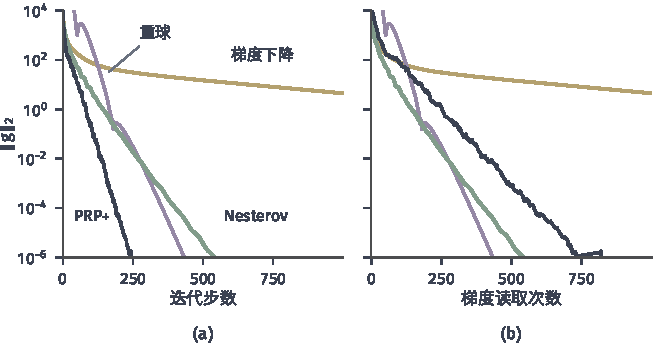
\includegraphics[width=112mm]{figures/05-optimization/02-smooth-optimization/matplotlib/fom-cost/figure.pdf}
  \caption{$100$维强凸非二次目标上的梯度大小，$\kappa=1001$，起点由固定种子的正态随机数给出。黄线是$\alpha=1/L$的梯度下降，紫线是按式~\eqref{eq:fom-hb-params}取参数的重球法，绿线是强凸参数的Nesterov方法，黑线是PRP+配合强Wolfe线搜索（$c_1=10^{-4}$，$c_2=0.1$）。(a)横轴是迭代步数。(b)横轴是梯度读取次数，同一组数据的位置变了。}
  \label{fig:fom-cost}
\end{BookInlineFigure}

按迭代步数，PRP+最少，$244$步，重球法$434$步，Nesterov方法$542$步，梯度下降$7574$步。按梯度读取，PRP+用了$821$次，比重球法的$435$次和Nesterov方法的$543$次都多。只看左图会选PRP+，只看右图会选重球法。

这张图也提醒另一点。重球法在这里表现好，但定理不保证它：目标不是二次的。Nesterov方法多读了约百分之二十五的梯度，换来的是对这一类目标有定理保证。四种配置中只有PRP+不需要$L$和$\mu$。这两个常数无法估计时，它可以直接运行；梯度下降配回溯也能做到这一点，只是更慢。

\paragraph{输出什么}
最后要说明报告哪个点。按定理~\ref{thm:fom-gd-nonconvex}的说法，非凸时应记录梯度最小的迭代点；凸与强凸的定理针对最后一个迭代点。Nesterov方法的目标差不单调，如果需要，可以另外保留函数值最低的点，这只需要在已经计算函数值时比较。

非线性共轭梯度的$\liminf$结论并不保证最后一点最好，同样应保留历史最优点。无论哪种方法，宣布达到精度之前都应该在输出点处重新计算一次梯度，而不是用外推点的梯度代替，后者并不是输出点的残差。

\section{本章小结}
\label{sec:fom-summary}

本章在只有函数值和梯度的条件下回答了“朝哪走、走多远、用不用历史”。负梯度是局部最陡的方向，二次上界决定一步能走多远，$\alpha=1/L$保证每步下降。梯度下降的保证按假设分三档：非凸时梯度变小，凸时目标差按$1/T$，强凸时按$(1-1/\kappa)^T$。

病态的目标让步长被陡峭方向限制，平坦方向进展缓慢，步数与$\kappa$成正比。历史位移可以把一致的方向累积起来，把振荡的方向抵消。重球法在当前点读取梯度，在正定二次目标上把各方向的收缩因子拉平为$(\sqrt\kappa-1)/(\sqrt\kappa+1)$，但这组参数离开二次目标可能循环。Nesterov方法把梯度移到外推点，用势函数得到强凸时的$(1-1/\sqrt\kappa)^T$和凸时的$1/T^2$，适用于一般的光滑目标，但函数值不必单调，目标非凸时定理不适用。

非线性共轭梯度保留上一方向，用线搜索决定步长，不需要曲率常数。FR配合$c_2<\tfrac12$的强Wolfe条件保证下降和$\liminf\lVert\bm{g}^{(t)}\rVert_2=0$，容易卡顿；PRP能自动重置，但需要PRP+、充分下降或重启等附加规则才能谈收敛。正定二次目标上的共轭性和有限步终止，在非线性目标上都不能照搬。

比较这些方法时，保证的条件和度量必须对应，成本要按梯度读取和线搜索试探计入，迭代次数少不等于总计算少。这些方法对局部曲率的利用都是间接的：历史位移和梯度差只是曲率的影子。如果能直接计算或近似局部曲率，更新方向可以由二次模型给出，下一章由此建立Newton方向。

